% GITCOMMIT: 37e4b23
\documentclass[12pt]{article}
\usepackage{t1enc} % as usual
\usepackage[T1]{fontenc}
\usepackage[utf8]{inputenc}
\usepackage{amsmath, amssymb, amsthm}
\usepackage{graphicx}
\usepackage{subfig}
\usepackage[numbers,sort&compress]{natbib}
\usepackage{hyperref}
\usepackage{geometry}\geometry{margin=1in}
\usepackage{lineno}\linenumbers
\usepackage{booktabs}
\usepackage[ruled,vlined]{algorithm2e}
\usepackage{listings}
\usepackage{xcolor}
\newtheorem{lemma}{Lemma}
\newtheorem{proposition}{Proposition}
\newtheorem{definition}{Definition}
\newtheorem{remark}{Remark}

\lstset{
  language=Python,
  basicstyle=\small\ttfamily,
  keywordstyle=\color{blue}\bfseries,
  commentstyle=\color{gray}\itshape,
  stringstyle=\color{teal},
  numberstyle=\tiny\color{gray},
  numbers=left,
  stepnumber=5,
  numbersep=8pt,
  frame=single,
  breaklines=true,
  breakatwhitespace=false,
  showspaces=false,
  showstringspaces=false,
  tabsize=4,
  captionpos=b,
}

\title{Noise Can Save a Sperm Parasite: \\Stochastic Stabilization in Gynogenetic Complexes}
\author{Juan B. Gutiérrez\textsuperscript{1}}
\date{
  \textsuperscript{1}University of Texas at San Antonio, San Antonio, Texas, USA\\
  \texttt{juan.gutierrez3@utsa.edu}
}

\begin{document}

\maketitle

%% =====================================================================
%% ABSTRACT
%% =====================================================================
\begin{abstract}
The Amazon molly (\textit{Poecilia formosa}) is a gynogenetic species that reproduces by sperm parasitism: females require sperm from males of a bisexual host species to initiate embryo development, but the paternal genome is not incorporated into offspring.  This creates a gynogenetic system in which unisexual females drive the host population toward feminization and potential extinction.  The puzzle of continued coexistence between \textit{P.~formosa} and its bisexual hosts has motivated mathematical models incorporating population-dependent male mate discrimination and environmental stochasticity.

We present a three-population model (bisexual females~$f$, males~$m$, unisexual females~$p$) with logistic growth and a sigmoid discrimination function, analyzed under three stochastic frameworks: (i)~a Random ODE (RODE) with piecewise-constant parametric noise, (ii)~an It\^{o} stochastic differential equation (SDE) with multiplicative geometric noise, and (iii)~a Stratonovich SDE with the same noise structure but different stochastic calculus convention.  Each SDE formulation is studied under two noise structures---common environmental noise (single Wiener process) and independent multiplicative noise (per-population Wiener processes)---yielding five formulations in total.

Our key results are: (a)~the speed of male mate discrimination governs the extinction/coexistence outcome across all five formulations, confirming the robustness of this ecological finding; (b)~the RODE boundary dissipativity condition ($\eta_f + \eta_m + \eta_p
< 3$) characterises phase-space contraction at the population ceiling and
has no exact SDE analog---the Stratonovich scalar Lyapunov exponent is noise-amplitude-independent, while the It\^{o} exponent is shifted by $-\sigma^2/2$; (c)~under mean-field moment closure, It\^{o} noise does not shift ensemble means but Stratonovich noise does, acting as an effective noise-induced birth rate increment of $+\tfrac{1}{2}\sigma_i^2 \mathbb{E}[\tilde{u}_i]$; (d)~under independent multiplicative noise the diffusion cross-driving between populations vanishes, though deterministic coupling can still generate covariance through the shared nonlinear drift.  These results demonstrate that formulation choice matters quantitatively for stability predictions but not qualitatively for the ecological conclusions, providing practical guidance for stochastic modeling of gynogenetic population dynamics.
\end{abstract}

%% =====================================================================
%% 1. INTRODUCTION
%% =====================================================================
\section{Introduction}
%% =====================================================================
% Paragraph 1 --- The ecological paradox
How can a sperm parasite coexist with its host when simple ecological logic predicts the parasite should drive the host to extinction, thereby destroying its own sperm supply and collapsing the entire system?  The logic of collapse is straightforward: each mating between a male and a parasitic female produces only parasitic offspring, so the growing parasite population diverts an increasing fraction of male mating effort away from conspecific females.  Fewer bisexual matings produce fewer males in the next generation, which reduces the sperm supply available to all females---parasite and host alike.  In the absence of any counteracting mechanism, the positive feedback loop drives the bisexual population to local extinction, after which the parasite, deprived of sperm, collapses as well.  Yet field data flatly contradict this prediction of inevitable collapse.  The gynogenetic fish \textit{Poecilia formosa} (the Amazon molly) has coexisted with its bisexual host species \textit{P.~mexicana} and \textit{P.~latipinna} across a wide range of habitats in southeastern Texas and northeastern Mexico for an evolutionary period estimated at more than 100{,}000 years~\citep{Avise1991}.  Understanding how this coexistence is maintained, despite the relentless demographic pressure toward feminization, is one of the central puzzles in the ecology of unisexual vertebrates.

% Paragraph 2 --- The biology of P. formosa
Unisexual reproduction has been documented in plants, invertebrates, and more than fifty vertebrate species.  Two mechanisms sustain all-female populations: parthenogenesis, in which embryo development occurs without fertilization, and gynogenesis, in which sperm from a male donor of a different species is necessary to initiate embryo development but the paternal genetic material is excluded from the offspring.  Species that reproduce by gynogenesis are termed \textit{sperm parasites}, and the sperm-donating species is the \textit{sperm host}~\citep{Kokko2008}.  The first gynogenetic vertebrate, \textit{P.~formosa}, was discovered by Hubbs and Hubbs in 1932~\citep{Hubbs1932}.  Molecular confirmation via mitochondrial DNA established that \textit{P.~mexicana} is the recent female parent of \textit{P.~formosa}~\citep{Avise1991}.  Field data from the Soto La Marina drainage in northeastern Mexico, gathered at 20 locations between 1970 and 1978, show a wide range of variation in the proportion of unisexuals relative to the total population from year to year, even at the same location~\citep{Balsano1989}.  The habitat varies from shallow water flowing over gravel with intermittent pools to turbid water flowing over a silty bottom; during the dry season only disconnected pools remain, and during the rainy season these pools reconnect.  This environmental oscillation between isolation and connectivity imposes stochastic variation with clear alternation between deleterious and additive effects on the population.  It is worth noting that \textit{P.~formosa} is mostly diploid; triploid XXY offspring can occur, but the Y chromosome remains silent and does not influence population dynamics~\citep{Balsano1989}.

% Paragraph 3 --- Prior mathematical models and their gaps
Several mathematical models have addressed gynogenetic population dynamics.  \citet{Kiester1981} created a generic sperm-dependent gynogenesis model applicable to a wide range of species and showed that a sexual discrimination factor is necessary to sustain the population; however, their model considers neither population-dependent discrimination dynamics nor the three-population structure specific to poeciliids.  \citet{Schley2004} developed a two-species model incorporating competition with Allee effects and showed that purely ecological factors can sustain coexisting populations, but their model does not include parasitism.  \citet{Peck1999} created a simulation model demonstrating that asexual takeover is likely in structured environments and concluded that migration and spatial fragmentation are important factors for sustaining bisexual populations, but did not address discrimination behavior.  \citet{Kokko2008} showed that spatial dynamics plays an important role in continued coexistence of gynogenetic complexes, though their model does not capture discrimination speed as a control variable.  \citet{Heubel2009} demonstrated that male mating efficiency and a sexual discrimination factor can stabilize a gynogenetic species complex, but used a fixed discrimination level rather than a population-dependent function.  None of these models account for two attributes observed in poeciliid field data: (i)~the high variability of unisexual proportions across locations and years, and (ii)~the role of the speed of male mate discrimination as a determinant of coexistence versus extinction.

% Paragraph 4 --- Male discrimination behavior
Male mate discrimination is one of the principal mechanisms proposed to explain coexistence between unisexuals and bisexuals~\citep{Kokko2008, Balsano1989, Kiester1981, Heubel2009}.  Males of the host species show a population-dependent selective preference for conspecific females: when the unisexual population is low, males mate with parasites at a frequency comparable to mating between bisexuals, but when the unisexual population is high, males strongly favor conspecific females~\citep{Riesch2008}.  Two explanations for this behavior exist in the literature.  The first is ``foreignness'': males are more willing to mate with unfamiliar females, so that when unisexuals are rare they are perceived as novel, but when unisexuals become common they lose this advantage~\citep{Balsano1989}.  The second is dominance hierarchies: dominant males show a marked preference for conspecific females, whereas small, subordinate males mate indiscriminately with both conspecifics and unisexuals~\citep{Balsano1989}.  Field observations indicate that bisexual poeciliids account for less than 20\% males in natural populations~\citep{Balsano1989, Snelson1980}, suggesting that the proportion of females in bisexual progeny is approximately $a \approx 0.8$.  The present model captures population-dependent discrimination through a sigmoid function $\gamma(p)$ that transitions smoothly from no heterospecific discrimination to strong conspecific preference as the parasite population grows.

% Paragraph 5 --- Stochastic modeling choice and contribution
The present study introduces three stochastic frameworks for the gynogenetic three-population model---a Random ODE (RODE) with piecewise-constant parametric noise, an It\^{o} SDE with multiplicative geometric noise, and a Stratonovich SDE with the same noise structure---and studies each SDE under two noise architectures: common environmental noise (a single Wiener process shared by all populations) and independent multiplicative noise (separate Wiener processes for each population), yielding five formulations in total.  The comparison matters because different biological interpretations of noise lead to different mathematical properties: RODE paths are smooth between resampling events, while SDE paths are nowhere differentiable; the It\^{o} integral evaluates the integrand at the left endpoint, while the Stratonovich integral uses the midpoint, producing different drift terms for multiplicative noise.  These are not merely technical distinctions---they carry biological consequences for stability predictions and extinction probability estimates.  The Wong-Zakai theorem establishes that when environmental forcing has finite correlation time, as is the case for seasonal flooding in the \textit{P.~formosa} habitat, the Stratonovich interpretation is the correct mathematical limit of smooth noise approximations~\citep{Oksendal2003}.  The choice of stochastic framework is therefore not a matter of convention but a modeling decision with quantitative implications.

% Paragraph 6 --- Paper structure
The remainder of this paper is organized as follows.  Section~2 presents the biological model, including the deterministic core equations, non-dimensionalization, and the sigmoid discrimination function.  Section~3 develops the three stochastic formulations and their interrelationships, including the It\^{o}--Stratonovich conversion and the empirical RODE-to-SDE calibration procedure.  Section~4 provides the analytical results: the RODE Dissipative Stochasticity Lemma, the SDE moment equations under mean-field closure, and the scalar Lyapunov exponent analysis for both It\^{o} and Stratonovich interpretations.  Section~5 presents numerical results for all five formulations, including ensemble statistics, moment equation validation, and stability boundary comparison.  Section~6 discusses the ecological and methodological implications, and Section~7 concludes with a summary of findings, their significance, and testable predictions for future work.


%% =====================================================================
%% 2. BIOLOGICAL MODEL
%% =====================================================================
\section{Biological Model}
%% =====================================================================

%---------------------------------------------------------------
\subsection{Mechanistic Derivation of the Mathematical Models}
%---------------------------------------------------------------

The dimensional model is constructed from first principles using the
mass-action framework~\citep{Buckingham:1914}, in which birth events arise
from encounters between individuals and the rate of each encounter type is
proportional to the product of the interacting population sizes.  The
derivation proceeds from four simplifying assumptions.

\begin{enumerate}
  \item \textbf{Common vital rates.}  All individuals, regardless of
    genotype, share a single per-capita birth coefficient $\tilde{\beta}$
    (proportional to offspring viability) and a single per-capita death
    coefficient $\tilde{\delta}$ (mortality from predation, disease, and
    senescence).

  \item \textbf{Sperm limitation.}  Sperm is the limiting resource in the
    mating pool.  A bisexual male allocates his total mating effort across
    all female encounters; the discrimination factor $\gamma \in (0,1]$
    defines the fraction of that effort directed toward unisexual females
    $\tilde{p}$.  The complementary fraction $(1-\gamma)$ is directed
    toward bisexual females $\tilde{f}$.  Consequently, the effective
    number of bisexual females competing for male mating effort is
    $\tilde{f} - \gamma\tilde{p}$: the total bisexual female population
    minus the portion of unisexuals that divert male attention.

  \item \textbf{Pedigree-determined offspring sex.}  From the mating
    pedigrees: (a)~a bisexual male--bisexual
    female encounter produces a fraction $a$ of female offspring and a
    fraction $(1-a)$ of male offspring; (b)~a bisexual male--unisexual
    female encounter produces only unisexual female offspring via
    gynogenesis, with no paternal genetic contribution to the progeny.

  \item \textbf{Logistic density dependence.}  All populations share the
    carrying capacity $\tilde{K}$, entering through the logistic factor
    $\tilde{L} = 1 - (\tilde{f}+\tilde{m}+\tilde{p})/\tilde{K}$, which
    limits total population growth as the system approaches its
    environmental ceiling.
\end{enumerate}

\noindent\textbf{Birth terms.}
Applying mass action to each mating type and invoking Assumptions 2--4,
the birth contribution to each population per unit time is:
%
\begin{align}
  \text{bisexual females born:}   &\quad
    a\,\tilde{\beta}\,\tilde{L}\,\tilde{m}\,(\tilde{f}-\gamma\tilde{p}),
    \label{eq:birth_f} \\[4pt]
  \text{bisexual males born:}     &\quad
    (1-a)\,\tilde{\beta}\,\tilde{L}\,\tilde{m}\,(\tilde{f}-\gamma\tilde{p}),
    \label{eq:birth_m} \\[4pt]
  \text{unisexual females born:}  &\quad
    \gamma\,\tilde{\beta}\,\tilde{L}\,\tilde{m}\,\tilde{p}.
    \label{eq:birth_p}
\end{align}
%
Equations~\eqref{eq:birth_f} and~\eqref{eq:birth_m} share the encounter
pool $(\tilde{f}-\gamma\tilde{p})$ because both bisexual sexes arise
exclusively from bisexual matings.  Equation~\eqref{eq:birth_p} has its
own encounter pool $\tilde{m}\tilde{p}$, scaled by $\gamma$, because every
sperm-triggered gynogenetic event between a male and a $P.~formosa$ female
produces only $P.~formosa$ offspring.

\noindent\textbf{Death terms.}
Each population declines at per-capita rate $\tilde{\delta}$, giving death
contributions $-\tilde{\delta}\tilde{f}$, $-\tilde{\delta}\tilde{m}$, and
$-\tilde{\delta}\tilde{p}$ respectively.

\noindent\textbf{The discrimination factor $\gamma$ and its dependence on
population context.}  In full generality, $\gamma$ is a function of two
population-level quantities: the parasite population size $\tilde{p}$ and
the male-to-female ratio $\rho = \tilde{m}/(\tilde{f}+\tilde{p})$.
The dependence on $\tilde{p}$ captures the well-documented
population-dependent preference of host males for conspecific females: when
$\tilde{p}$ is small, males encounter few unisexuals and mate
indiscriminately ($\gamma \approx \gamma_o$); when $\tilde{p}$ is large,
males strongly avoid unisexuals ($\gamma \approx \gamma_\infty$)
\citep{Balsano1989}.  The dependence on $\rho$ reflects a second
behavioral mechanism: \citet{Riesch2008} report, following field sampling
across five Texas sites throughout the breeding season, that males become
less discriminating as they become proportionally rare relative to the
total female pool---a pattern consistent with earlier observations in the
bark beetle \textit{Ips acuminatus}~\citep{Loyning1996}.  Mechanistically,
a male facing a high per-capita encounter load bears a greater cost of
rejecting any female, which erodes the discrimination threshold.

The present analysis adopts the biologically motivated reduction
$\gamma = \gamma(\tilde{p})$, treating the male-to-female ratio as a
source of model uncertainty rather than an explicitly parameterized
feedback.  This reduction is justified on two grounds.  First, the
Riesch data are observational rather than experimental: the seasonal
decline in sperm acquisition is confounded with late-season reproductive
physiology and cannot, from available data alone, be used to calibrate an
independent $\rho$-response function.  Second, and importantly, the
Riesch field data show that discrimination against $P.~formosa$ persists
even when males are exceedingly rare late in the season, indicating that
the $\tilde{p}$-dependent mechanism is the dominant effect and the
$\rho$-dependent modulation is secondary.  The consequences of
incorporating the full $\gamma(\tilde{p}, \rho)$ structure are discussed
in Section~\ref{sec:discussion} as a testable extension of the model.

\noindent\textbf{The dimensional system.}
Combining birth and death contributions from
Equations~\eqref{eq:birth_f}--\eqref{eq:birth_p} yields the
dimensional system:
%
\begin{align}
  \frac{d\tilde{f}}{dt} &=
    a\,\tilde{\beta}\,\tilde{L}\,\tilde{m}
    \!\left(\tilde{f}-\gamma\tilde{p}\right)
    - \tilde{\delta}\,\tilde{f},
    \label{eq:dim_f}\\[4pt]
  \frac{d\tilde{m}}{dt} &=
    (1-a)\,\tilde{\beta}\,\tilde{L}\,\tilde{m}
    \!\left(\tilde{f}-\gamma\tilde{p}\right)
    - \tilde{\delta}\,\tilde{m},
    \label{eq:dim_m}\\[4pt]
  \frac{d\tilde{p}}{dt} &=
    \gamma\,\tilde{\beta}\,\tilde{L}\,\tilde{m}\,\tilde{p}
    - \tilde{\delta}\,\tilde{p},
    \label{eq:dim_p}\\[4pt]
  \tilde{L} &= 1 - \frac{\tilde{f}+\tilde{m}+\tilde{p}}{\tilde{K}},
    \notag
\end{align}
%
where tildes denote dimensional quantities throughout.
Stochastic perturbations $\tilde{\eta}_i(t)$ are appended to each
equation in Section~\ref{sec:stochastic}; the deterministic skeleton
above is analysed first to establish the equilibrium structure.
The system is non-dimensionalized in Section~\ref{sec:nondim}.

% %---------------------------------------------------------------
% \subsection{Mechanistic Derivation of the Mathematical Models}
% %---------------------------------------------------------------
%   The construction of a Trojan Y Chromosome mathematical model uses the principle of mass action. This framework is based upon the interaction of gametes within a population of mating individuals, and provides a means to derive the equations used in the Trojan Y Chromosome ordinary differential equation model.
  
% Consider the population as a mixture of fish with different genotypes, each contributing their gametes to a common mating pool. The progeny arising from this common mating pool at each generation could be calculated provided that  (i) the fraction of each parental genotype in the population is known, and (ii) the distribution of different progeny genotypes is known for each of the possible mating pairs in the population. In this approach, the population is considered as a collection of different Punnet Squares, each representing a mating.  By knowing the frequency that each parent occurs within each Punnet Square, we can calculate the distribution of progeny genotypes for the common mating pool. We can then apply this distribution to the new births that are expected at each generation giving us the exact number of new fish (births) expected for each genotype. 

% The initial population consists of only males ($m$) and females ($f$) (two genotypes XY and XX, and one possible mating pair), and with even sex ratios, none of the sexes can have a population greater than half the carrying capacity $K$, i.e. $f \leq K/2$, and $m \leq K/2$ for all times. The number of females in the next generation is:
% \begin{align*}\label{eq:f1}
% Population_{t+\Delta t} & = Population_{t} + Logistic * Mating - Death  \\
% f_{t+\Delta t} & = f_t + L(f,m) M(f,m) \Delta t - \delta f_t \Delta t,
% \end{align*}
% where $L(f,m)$ is a density-dependent logistic term such that $L(f,m) = 0$ when $f = K/2$ and $m = K/2$; $L(f,m) \approx 1$ when $f$ and $m$ are at their minimum values. Then,
% \[
% L(f,m) = \left(K - f_t - m_t \right) \frac{1}{K} = \left( 1 - \frac{f_t+m_t}{K} \right). 
% \] 
% $M(f,m)$ is a mating function that determines the number of new individuals for each genotype at each time step
% \[
% M(f,m) = BirthRate * Population * ProgenyProbability *FemaleParentProbability * MaleParentProbability
% \] 	

% In the TYC system there are two types of females ($f$ and $r$) and two types of males ($m$ and $s$). The new $f$ individuals arise only from the matings involving $f$ and $m$ and comprise one half of the progeny. The fraction of the total females contributing to the gamete pool that are $f$  ($FemaleParentProbability$) and the fraction of total males contributing to the gamete pool that are $m$ ($MaleParentProbablitity$) are 
% \[
% \frac{f_t}{f_t+r_t} \mbox{ and }  \frac{m_t}{m_t+s_t}
% \]
% respectively. If $P$ represents total population, and $\omega$ is a birth rate, the mating function for $f$ in the TYC system is
% \[
% M(f_t,m_t,s_t,r_t) =  \omega P  \frac{1}{2}\frac{f_t}{f_t+r_t}  \frac{m_t}{m_t+s_t}, 
% %M(f,m) & = \omega P \frac{f_t}{f_t} \frac{m_t}{m_t}. 
% \]
% and the TYC logistic term becomes
% \begin{align*}
% L(f_t,m_t,r_t,s_t) = & \left(K - f_t - m_t - s_t - r_t \right) \frac{1}{K} \\ 
%                     =  & \left( 1 - \frac{f_t+m_t+s_t+r_t}{K} \right). 
% \end{align*} 

% The number of $f$ in the next generation is given by 
% \begin{align*}
% f_{t+\Delta t} = & f_t + \omega P \left( \frac{1}{2}\frac{f_t}{f_t+r_t}  \frac{m_t}{m_t+s_t} \right) L \Delta t- \delta f_t \Delta t.
% \end{align*} 
% The term $f_t+r_t$ in the denominator represents the total number of females. Let $\alpha$ be the percentage of females in the population; then, $f_t+r_t = \alpha P$, $m_t+s_t = (1- \alpha) P$ and 
% \begin{align*}
% f_{t+\Delta t} = & f_t +  \frac{\omega P}{\alpha P (1-\alpha)P} \frac{1}{2}f_t m_t L \Delta t - \delta f_t \Delta t\\ 								 
%                 = & f_t + \frac{\omega}{\alpha (1-\alpha)P} \frac{1}{2} f_t m_t L \Delta t - \delta f_t \Delta t	
% \end{align*} 
% We can use two asymptotic estimates: (i) the \textit{a priori} estimate $f \rightarrow 0$ as $t \rightarrow  \infty$ if enough $r$ are added to the population, (ii) the steady state for $r$ is $\mu/\delta$, and (iii) the fundamental assumption is that the population is kept at the carrying capacity, therefore $P \approx K$, to determine that $\alpha \rightarrow  \frac{\mu/\delta}{K}$, which is a constant. Then, let
% \[
% \beta = \frac{\omega}{\alpha (1-\alpha)K} = \frac{\omega}{\frac{\mu/\delta}{K} \left( 1 - \frac{\mu/\delta}{K} \right) K} = \frac{\omega \delta}{\mu\left( 1 - \frac{\mu}{ \delta K} \right) } 
% \]
% Taking the limit as $\Delta t \rightarrow 0$, 
% \begin{align*}
% \lim_{\Delta t \rightarrow 0} \frac{f_{t+\Delta t} - f_t}{\Delta t} = \frac{df}{dt} = \frac{1}{2} \beta f m L - \delta f_t,
% \end{align*}
% which is the same as Equation \ref{eq:fTYC} in the TYC model. The equations for the other genotypes in the TYC and DC models are produced in the same way. 


%---------------------------------------------------------------
\subsection{Deterministic Core}\label{sec:deterministic}
%---------------------------------------------------------------

The dimensional system derived in the preceding subsection,
Equations~\eqref{eq:dim_f}--\eqref{eq:dim_p}, is analysed here in the
deterministic limit $\tilde{\eta}_i \equiv 0$ and with $\gamma =
\text{constant}$.  The steady state satisfies
$\dot{\mathbf{u}}(\mathbf{u}_0) = \mathbf{0}$.  Solving the resulting
algebraic system yields the unique equilibrium discrimination factor:
\begin{equation}\label{eq:GammaSS}
  \gamma_{eq} = \frac{a f^*}{a p^* + f^*}.
\end{equation}
With the parameter values $a = 0.8$, $f^* = 100$, and
$p^* = 10$, this gives $\gamma_{eq} = 80/108 \approx 0.74$.
Three qualitative regimes exist: when $\gamma < \gamma_{eq}$, unisexuals
go extinct; when $\gamma = \gamma_{eq}$, coexistence obtains; when
$\gamma > \gamma_{eq}$, bisexuals go extinct followed by unisexuals.

When $\gamma p > f$, the term $f - \gamma p$ becomes negative,
representing a net diversion of male mating effort so complete that it
exceeds the available bisexual female population; in this regime the model
predicts net decline of the bisexual population from competition for male
attention alone.  The numerical implementation clips populations to
nonnegative values at each step to maintain biological feasibility.


%---------------------------------------------------------------
\subsection{Non-Dimensionalization}\label{sec:nondim}
%---------------------------------------------------------------

Non-dimensionalization reduces the number of independent parameters and
reveals the natural scales of the problem~\citep{Buckingham:1914}.
Stochastic perturbations to the per-capita growth rates are introduced at
this stage as dimensionless noise amplitudes $\eta_i(t) =
\tilde{\eta}_i(t)/\tilde{\delta}$; their statistical properties and
biological interpretation are developed in Section~\ref{sec:stochastic}.  The system is non-dimensionalized via $u_i = \tilde{u}_i/\tilde{K}$, $\tau = \tilde{\delta}\,t$, $\beta = \tilde{\beta}\tilde{K}/\tilde{\delta}$, and $\eta_i = \tilde{\eta}_i/\tilde{\delta}$, yielding
\begin{align}
  \frac{df}{d\tau} &= a \beta L m(f-\gamma p) - (1-\eta_f) f, \label{eq:PoeciliaF} \\
  \frac{dm}{d\tau} &= (1-a) \beta L m(f-\gamma p) - (1-\eta_m) m, \label{eq:PoeciliaM} \\
  \frac{dp}{d\tau} &= \gamma\beta L m p - (1-\eta_p) p, \label{eq:PoeciliaP}
\end{align}
where $L = 1-(f+m+p)$ and all quantities are dimensionless.  The non-dimensional death rate is $\delta = 1$ by construction.  With the parameter values in Table~\ref{tab:parameters}, $\beta = 0.1 \times 300 / 0.1 = 300$, and the discrimination speed becomes $v_{\text{nondim}} = v \tilde{K}$ (so $v_{\text{fast}} = 60$, $v_{\text{slow}} = 6$).  Non-dimensional time $\tau = 20$ corresponds to dimensional $t = 200$.


%---------------------------------------------------------------
\subsection{Sexual Discrimination Function}
%---------------------------------------------------------------

The simplified case $\gamma = $ constant is unrealistic.  A population-dependent sigmoid function provides a better approximation to the observed behavior, allowing a smooth transition from no heterospecific discrimination ($\gamma_o$) to maximum heterospecific discrimination ($\gamma_\infty$) with a nearly linear central regime:
\begin{equation}\label{eq:DiscriminationFactor}
  \gamma(p) = \frac{\gamma_o - \gamma_\infty}{1+e^{vp-r}} + \gamma_\infty,
\end{equation}
where $\gamma_o = 1$ is the initial discrimination (no preference), $\gamma_\infty = 0.2$ is the asymptotic discrimination (20\% mating with unisexuals), $v > 0$ is the speed of male mate discrimination, and $r = 5$ shifts the sigmoid.  The asymptotic value $\gamma_\infty = 0.2$ corresponds to the range of parameters reported by \citet{Riesch2008} and \citet{Balsano1989}; it is used to illustrate the behavior of the system and should not be considered an intrinsic fixed property.  Figure~\ref{fig:gamma_curves} shows curves for three discrimination speeds.  The parameter $v$ plays a pivotal role: slow discrimination ($v = 0.02$) leads to extinction, while fast discrimination ($v = 0.20$) leads to coexistence.

\begin{figure}[htbp]
  \centering
  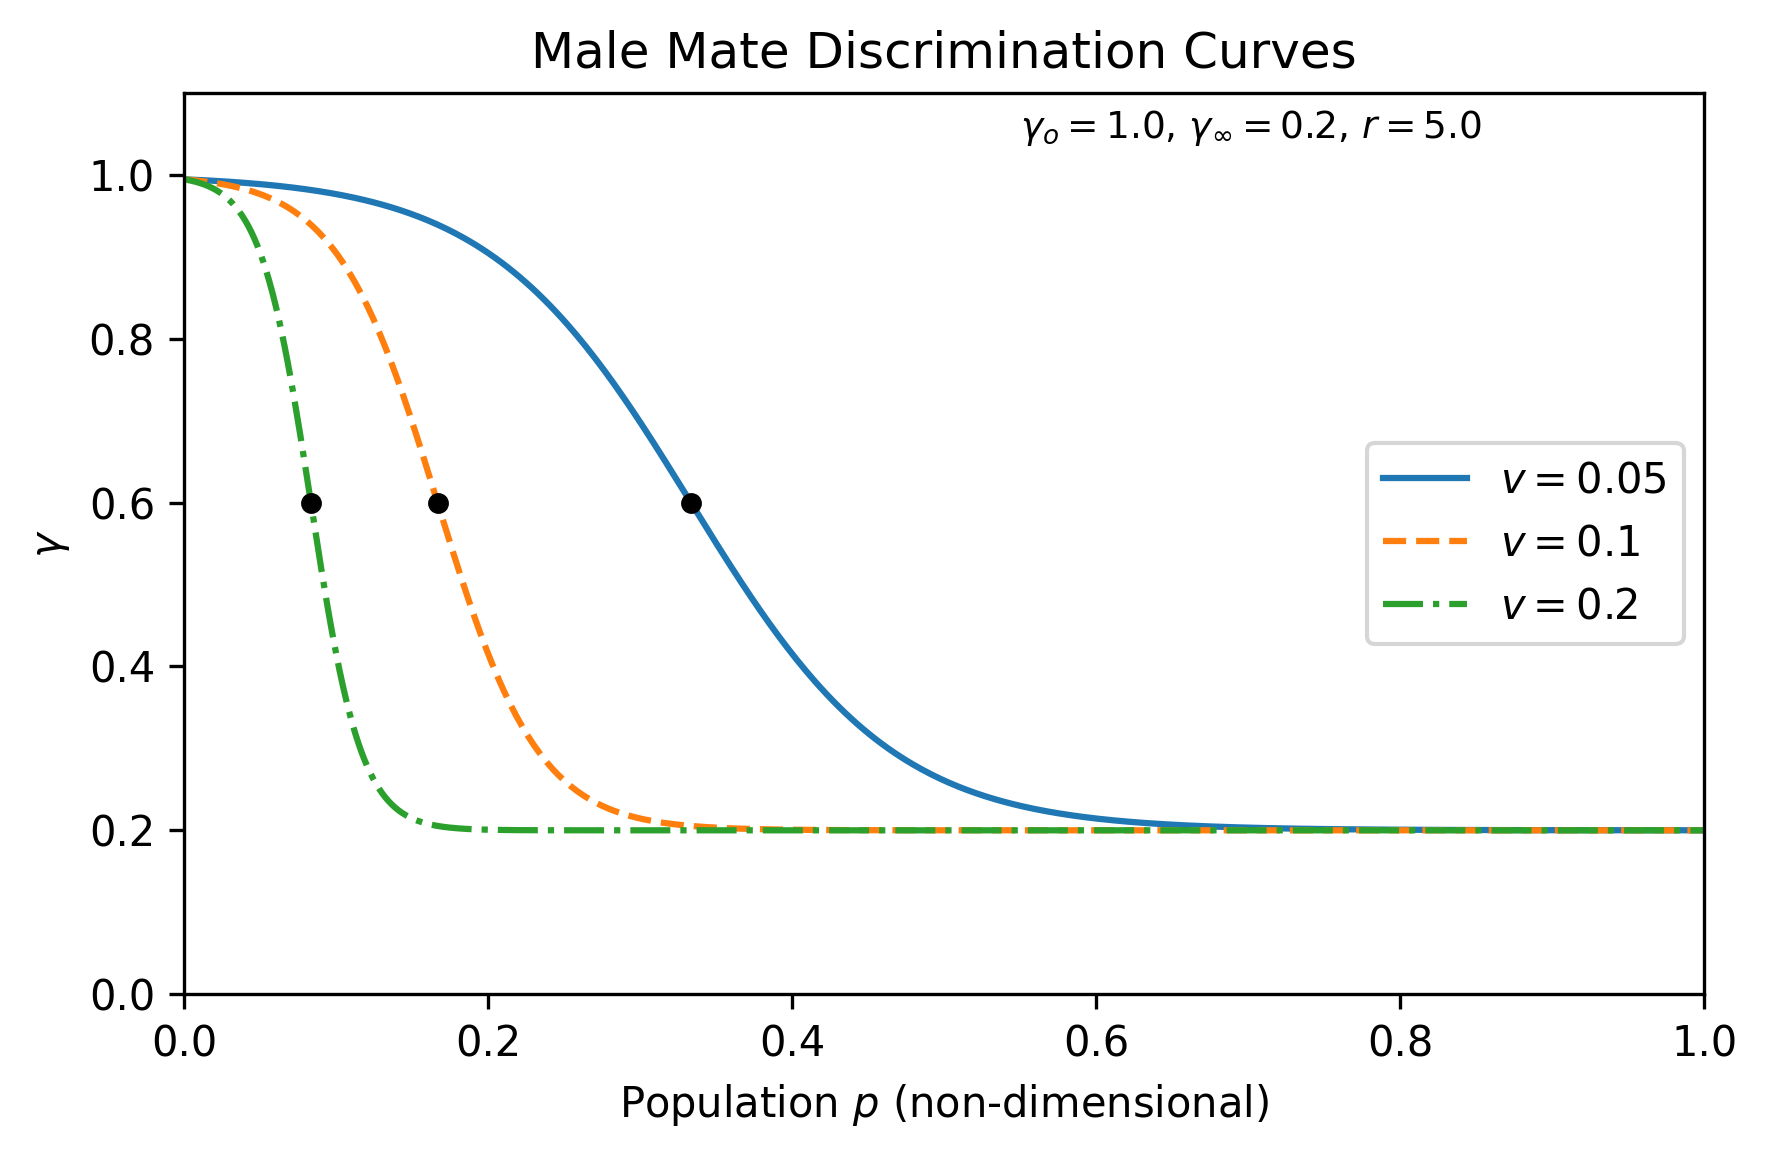
\includegraphics[width=0.6\textwidth]{poecilia_sde/figures/fig01_gamma_curves.png}
  \caption{Male mate discrimination curves for three speeds $v = 0.05$, $0.10$, $0.20$.  Parameters: $\gamma_o = 1$, $\gamma_\infty = 0.2$, $r = 5$.  Black dots mark inflection points.}
  \label{fig:gamma_curves}
\end{figure}


%% =====================================================================
%% 3. STOCHASTIC FORMULATIONS
%% =====================================================================
\section{Stochastic Formulations}\label{sec:stochastic}
%% =====================================================================
%---------------------------------------------------------------
\subsection{Random ODE (RODE) Formulation}
%---------------------------------------------------------------

The RODE formulation models environmental stochasticity through piecewise-constant random perturbations $\tilde{\eta}_i(t) \sim \mathrm{Uniform}[0, \tilde{\eta}_{\max}]$, resampled at each time step.  The noise enters multiplicatively as $\tilde{\eta}_i(t) \tilde{u}_i$, representing environmental surplus or deficit: when $\tilde{\eta}_i > \tilde{\delta}$, the population experiences net growth beyond deterministic rates.

This is a \emph{Random ODE}, not an SDE in the It\^{o}/Stratonovich sense: between resampling events, the system is a standard ODE, and classical Runge-Kutta methods (specifically, the Dormand-Prince RK45 pair via \texttt{solve\_ivp}) are appropriate solvers.  The RODE formulation produces bounded noise variance on each interval, in contrast to the unbounded diffusion of SDEs.

Experimental data on fish association in populations containing \textit{P.~formosa} show that bisexual females associate preferentially in small groups of their own kind, and dominant males direct approximately one third of their activity toward females with preference for conspecifics~\citep{Balsano1989}.  These spatial clustering patterns create a population-dependent bias in exposure to environmental perturbations: bisexual populations cluster more tightly and are less exposed to stochastic effects than \textit{P.~formosa}.  To reflect this, the noise amplitudes are structured as $\tilde{\eta}_f = \tilde{\eta}_m = (2/3)\tilde{\eta}$ and $\tilde{\eta}_p = \tilde{\eta}$.

\begin{remark}
The uniform distribution $\tilde\eta_i(t)\sim\mathrm{Uniform}[0,\tilde\eta_{\max}]$
has positive mean $\mathbb{E}[\tilde\eta_i]=\tilde\eta_{\max}/2$, so the RODE
introduces both variance and a positive mean growth bias compared to a
mean-zero noise model.  For the parameter values used here
($\tilde\eta_{\max}=0.1$, $\tilde\delta=0.1$ in the dissipative case),
the mean noise contribution equals the death rate; in the
threshold-exceeding case ($\tilde\eta_{\max}=0.25$) it exceeds it.
This positive bias is a feature of the random-environment model: it
represents a habitat whose average condition favours growth above the
baseline death rate.  Comparisons between RODE trajectories and SDE
trajectories therefore reflect both differences in stochastic formalism
and differences in mean drift; this distinction is acknowledged
throughout the Results.
\end{remark}


%---------------------------------------------------------------
\subsection{It\^{o} SDE Formulation}
%---------------------------------------------------------------

The It\^{o} SDE formulation replaces the piecewise-constant RODE noise with continuous multiplicative geometric noise driven by Wiener processes.  Two noise structures are considered.

% Common environmental noise
A single Wiener process $W(t)$ represents a shared habitat driver affecting all populations simultaneously:
\begin{align}
  d\tilde{f} &= \mu_f(\tilde{\mathbf{u}})\,dt + \sigma_f \tilde{f}\,dW, \label{eq:ItoCommonF} \\
  d\tilde{m} &= \mu_m(\tilde{\mathbf{u}})\,dt + \sigma_m \tilde{m}\,dW, \\
  d\tilde{p} &= \mu_p(\tilde{\mathbf{u}})\,dt + \sigma_p \tilde{p}\,dW,
\end{align}
where $\mu_i$ denotes the deterministic drift.

% Independent multiplicative noise
Separate Wiener processes $W_f$, $W_m$, $W_p$ model independent multiplicative fluctuations in each population:
\begin{align}
  d\tilde{f} &= \mu_f(\tilde{\mathbf{u}})\,dt + \sigma_f \tilde{f}\,dW_f, \\
  d\tilde{m} &= \mu_m(\tilde{\mathbf{u}})\,dt + \sigma_m \tilde{m}\,dW_m, \\
  d\tilde{p} &= \mu_p(\tilde{\mathbf{u}})\,dt + \sigma_p \tilde{p}\,dW_p.
\end{align}

The geometric multiplicative noise structure $\sigma_i \tilde{u}_i\,dW$ ensures near-zero positivity; numerical positivity is enforced via nonnegative clipping ($\tilde{u}_i = \max(\tilde{u}_i, 0)$) after each Euler-Maruyama step.

\begin{algorithm}[H]
\DontPrintSemicolon
\SetAlgoLined
\KwIn{Parameters $\sigma_f, \sigma_m, \sigma_p$, time step $\Delta t$, end time $T$, initial condition $\mathbf{u}_0$}
\KwOut{Solution trajectory $\mathbf{u}(t)$}
$\mathbf{u} \leftarrow \mathbf{u}_0$\;
\For{$n = 0, 1, \ldots, T/\Delta t - 1$}{
  $\Delta W \leftarrow \mathcal{N}(0, \sqrt{\Delta t})$ \tcp*{single increment for common; 3 for independent}
  $\boldsymbol{\mu} \leftarrow$ \texttt{txc\_rhs}$(t_n, \mathbf{u})$\;
  $\mathbf{u} \leftarrow \mathbf{u} + \boldsymbol{\mu}\,\Delta t + \boldsymbol{\sigma} \odot \mathbf{u} \odot \Delta\mathbf{W}$\;
  $\mathbf{u} \leftarrow \max(\mathbf{u}, 0)$ \tcp*{nonnegative clipping}
}
\caption{Euler-Maruyama method (It\^{o} SDE)}
\label{alg:EM}
\end{algorithm}

Population values are clipped to $[0, \infty)$ after each step, and the
logistic factor is evaluated as $L = \max(1 - f - m - p,\, 0)$; the
simulated system therefore solves a truncated approximation to the smooth
analytical model.


%---------------------------------------------------------------
\subsection{Stratonovich SDE Formulation}
%---------------------------------------------------------------
The Stratonovich formulation replaces the It\^{o} integral with the Stratonovich (mid-point) integral:
\begin{equation}
  d\tilde{f} = \mu_f\,dt + \sigma_f \tilde{f} \circ dW.
\end{equation}

The Wong-Zakai theorem justifies this choice: when noise represents a physical environmental process with finite but small correlation time, the Stratonovich interpretation is the correct limit of a smooth approximation~\citep{Oksendal2003}.  For \textit{P.~formosa}, seasonal flooding and connectivity changes in the Soto La Marina drainage have finite correlation time (on the order of weeks to months), the Stratonovich interpretation is natural when the environmental noise
arises as the white-noise limit of smooth fast-varying forcing; for
environmental drivers with longer correlation times an explicit
random-environment (RODE-type) model may be more appropriate.

The Heun method (explicit 2-stage predictor-corrector) is used, which converges to the Stratonovich integral:

\begin{algorithm}[H]
\DontPrintSemicolon
\SetAlgoLined
\KwIn{Parameters, $\Delta t$, $T$, $\mathbf{u}_0$}
\KwOut{Solution trajectory $\mathbf{u}(t)$}
$\mathbf{u} \leftarrow \mathbf{u}_0$\;
\For{$n = 0, 1, \ldots, T/\Delta t - 1$}{
  $\Delta W \leftarrow \mathcal{N}(0, \sqrt{\Delta t})$\;
  $\mathbf{g} \leftarrow \boldsymbol{\sigma} \odot \mathbf{u}$ \tcp*{diffusion at current state}
  $\bar{\mathbf{u}} \leftarrow \max(\mathbf{u} + \mathbf{g} \odot \Delta\mathbf{W},\, 0)$ \tcp*{predictor}
  $\bar{\mathbf{g}} \leftarrow \boldsymbol{\sigma} \odot \bar{\mathbf{u}}$ \tcp*{diffusion at predictor}
  $\boldsymbol{\mu} \leftarrow$ \texttt{txc\_rhs}$(t_n, \mathbf{u})$\;
  $\mathbf{u} \leftarrow \max\!\bigl(\mathbf{u} + \boldsymbol{\mu}\,\Delta t + \tfrac{1}{2}(\mathbf{g} + \bar{\mathbf{g}}) \odot \Delta\mathbf{W},\, 0\bigr)$\;
}
\caption{Heun method (Stratonovich SDE)}
\label{alg:Heun}
\end{algorithm}

Population values are clipped to $[0, \infty)$ after each step, and the
logistic factor is evaluated as $L = \max(1 - f - m - p,\, 0)$; the
simulated system therefore solves a truncated approximation to the smooth
analytical model.


%---------------------------------------------------------------
\subsection{Relationship Between Formulations}
%---------------------------------------------------------------
For geometric multiplicative noise, the Stratonovich-to-It\^{o} conversion introduces a drift correction.  The general conversion theorem states that if a scalar Stratonovich SDE has the form $dX = \mu\,dt + g(X)\circ dW$, the equivalent It\^{o} SDE is $dX = [\mu + \tfrac{1}{2}g(X)g'(X)]\,dt + g(X)\,dW$~\citep{Oksendal2003}.  Since the diffusion coefficient in our system is $g_i(\tilde{u}_i) = \sigma_i \tilde{u}_i$, we have $g_i'(\tilde{u}_i) = \sigma_i$, and the correction for each component is
\begin{equation}
  \frac{1}{2} g_i \frac{\partial g_i}{\partial \tilde{u}_i} = \frac{1}{2} \sigma_i^2 \tilde{u}_i.
\end{equation}
Therefore, the It\^{o}-equivalent drift of the Stratonovich system is:
\begin{align}
  \mu_f^{\text{It\^{o}-equiv}} &= a\beta L m(f - \gamma p) - \delta f + \tfrac{1}{2}\sigma_f^2 f, \\
  \mu_m^{\text{It\^{o}-equiv}} &= (1-a)\beta L m(f - \gamma p) - \delta m + \tfrac{1}{2}\sigma_m^2 m, \\
  \mu_p^{\text{It\^{o}-equiv}} &= \gamma\beta L m p - \delta p + \tfrac{1}{2}\sigma_p^2 p.
\end{align}
The correction term $+\tfrac{1}{2}\sigma_i^2 \tilde{u}_i$ is positive for all $\tilde{u}_i > 0$.  Because this correction enters additively with the same sign as the birth rate, it acts as an effective noise-induced birth rate increment.  Populations modeled under Stratonovich noise therefore experience a systematic upward bias in their drift relative to the same populations under It\^{o} noise.  These expressions are confirmed by symbolic verification (Appendix~A).

\begin{remark}[Noise-induced growth bias]
Under mean-field closure, It\^{o} noise does not shift ensemble means---the additional stochastic integral has zero expectation.  Stratonovich noise shifts means upward by $+\tfrac{1}{2}\sigma_i^2 \mathbb{E}[\tilde{u}_i]$, which acts as an effective noise-induced birth rate increment.  This is the key qualitative difference between the two calculi for the gynogenetic system.
\end{remark}


%---------------------------------------------------------------
\subsection{RODE-to-SDE Correspondence and Calibration}
%---------------------------------------------------------------
The RODE and SDE formulations are not related by a simple parameter substitution.  The RODE produces bounded noise on each interval (uniform on $[0, \tilde{\eta}_{\max}]$), while SDE variance grows as $\sigma^2 \mathbb{E}[\tilde{u}^2] t$.  Consequently, direct parameter comparison is impossible, which is itself a finding that motivates the Monte Carlo stability comparison in Section~5.

To enable visual comparison, we employ an empirical calibration procedure:
\begin{enumerate}
  \item Run a RODE ensemble ($n = 200$ paths) and compute $\text{Std}[\tilde{f}(T/2)]$.
  \item Binary search on $\sigma$ (SDE common noise) to match this standard deviation using a 100-path SDE ensemble.
  \item Record calibrated $\sigma$ values (Table~\ref{tab:calibration}).
\end{enumerate}


%% =====================================================================
%% 4. ANALYSIS
%% =====================================================================
\section{Analysis}
%% =====================================================================
%---------------------------------------------------------------
\subsection{RODE: Boundary Dissipativity Lemma}
%---------------------------------------------------------------

The following result characterizes the dissipative behavior of the RODE system at the population ceiling.  It applies specifically to the RODE formulation---a pathwise, Liouville-based phase-space contraction argument---and does not extend directly to It\^{o} or Stratonovich SDEs.

\begin{lemma}[RODE Boundary Dissipativity Lemma]\label{lem:DissipativePoecilia}
On the population ceiling $f+m+p=1$, the non-dimensional RODE system satisfies
$\nabla\cdot\mathbf{F} \le \eta_f(t)+\eta_m(t)+\eta_p(t)-3$.
In particular, the system is dissipative on that face whenever
$\eta_f(t)+\eta_m(t)+\eta_p(t)<3$.
\end{lemma}

\begin{proof}
We establish that $\nabla\cdot\mathbf{F} < 0$ on the population ceiling
$f+m+p=1$.  On this face the logistic factor $L = 1-f-m-p = 0$, so every
birth term vanishes---each contains $L$ as a multiplicative factor.  The
non-dimensional system therefore reduces to the pure death system
$\dot{f}=-(1-\eta_f)f$, $\dot{m}=-(1-\eta_m)m$, $\dot{p}=-(1-\eta_p)p$
augmented by the logistic structure.  More precisely, at any point on the
face we compute the partial derivatives using the product rule with
$\partial L/\partial f = \partial L/\partial m = \partial L/\partial p = -1$:
\begin{align}
  \frac{\partial\dot{f}}{\partial f}\bigg|_{L=0}
    &= a\beta m\bigl[0 - (f-\gamma p)\bigr] - (1-\eta_f)
     = -a\beta m(f-\gamma p) - (1-\eta_f), \\
  \frac{\partial\dot{m}}{\partial m}\bigg|_{L=0}
    &= (1-a)\beta m\bigl[0 - (f-\gamma p)\bigr] - (1-\eta_m)
     = -(1-a)\beta m(f-\gamma p) - (1-\eta_m), \\
  \frac{\partial\dot{p}}{\partial p}\bigg|_{L=0}
    &= \gamma\beta m\bigl[0 - p\bigr] - (1-\eta_p)
     = -\gamma\beta mp - (1-\eta_p).
\end{align}
Summing these three contributions:
\begin{equation}\label{eq:divF_face}
  \nabla\cdot\mathbf{F}\big|_{f+m+p=1}
  = -\beta m\bigl[(f-\gamma p)+(1-a)(f-\gamma p)/a \cdot a + \gamma p\bigr]
    - 3 + \eta_f+\eta_m+\eta_p.
\end{equation}
Collecting the $m$-bracket:
$a(f-\gamma p)+(1-a)(f-\gamma p)+\gamma p = (f-\gamma p)+\gamma p = f$, so
\begin{equation}\label{eq:BetaFactorPoecilia}
  \nabla\cdot\mathbf{F}\big|_{f+m+p=1} = -\beta m f - 3 + \eta_f+\eta_m+\eta_p.
\end{equation}
Since $\beta>0$, $m\ge 0$, and $f\ge 0$ throughout the feasible region, the
term $-\beta mf \le 0$.  Therefore
\begin{equation}
  \nabla\cdot\mathbf{F}\big|_{f+m+p=1}
  \;\le\; -3 + \eta_f+\eta_m+\eta_p,
\end{equation}
with equality on the edges $\{f=0\}$ or $\{m=0\}$ of the ceiling face.
This upper bound is negative if and only if $\eta_f+\eta_m+\eta_p < 3$.

\begin{remark}
This result is specific to the population ceiling $f+m+p=1$.  In the
interior of the feasible simplex where $L>0$, the birth terms contribute
positive terms to $\nabla\cdot\mathbf{F}$, and the condition
$\eta_f+\eta_m+\eta_p<3$ does not imply global phase-space contraction.
The boundary result is the ecologically meaningful condition: it governs
whether stochastic fluctuations that drive populations toward the
carrying capacity are dissipated (absorbed back) or amplified.
\end{remark}
\end{proof}

\begin{definition}
The state of the gynogenetic system when $\eta_f(t)+\eta_m(t)+\eta_p(t)<3$ is called a \textit{state of dissipative stochasticity}.
\end{definition}

\begin{definition}
The state of the gynogenetic system when $\eta_f(t)+\eta_m(t)+\eta_p(t)>3$ is called a \textit{state of non-dissipative stochasticity}.
\end{definition}

\begin{definition}
The state of the gynogenetic system when $\eta_f(t)+\eta_m(t)+\eta_p(t)=3$ is the \textit{dissipative threshold}.
\end{definition}


%---------------------------------------------------------------
\subsection{SDE: Moment Equations}
%---------------------------------------------------------------

We derive diffusion-approximated moment equations by applying It\^{o}'s lemma and the mean-field closure approximation $\mathbb{E}[u_i u_j] \approx \mathbb{E}[u_i]\mathbb{E}[u_j]$.  Let $F = \mathbb{E}[f]$, $M = \mathbb{E}[m]$, $P = \mathbb{E}[p]$.

\begin{proposition}[Mean equations, It\^{o}]\label{prop:ito_means}
Under mean-field closure, the ensemble means $(F, M, P)$ of the It\^{o} SDE system (with either noise structure) satisfy the deterministic ODE:
\begin{align}
  \frac{dF}{dt} &= a\beta(1-F-M-P)M(F - \gamma P) - \delta F, \\
  \frac{dM}{dt} &= (1-a)\beta(1-F-M-P)M(F - \gamma P) - \delta M, \\
  \frac{dP}{dt} &= \gamma\beta(1-F-M-P)MP - \delta P.
\end{align}
\end{proposition}

\begin{proof}
We begin by stating what It\^{o}'s lemma says in general form.  If $X_t$ satisfies an It\^{o} SDE $dX_t = \mu(X_t)\,dt + g(X_t)\,dW_t$, and $h(x)$ is a twice continuously differentiable function, then
\begin{equation}
  dh(X_t) = \left[\mu(X_t)h'(X_t) + \tfrac{1}{2}g^2(X_t)h''(X_t)\right]dt + g(X_t)h'(X_t)\,dW_t.
\end{equation}
We apply this to the identity function $h(f) = f$, for which $h'(f) = 1$ and $h''(f) = 0$.  Since the It\^{o} SDE for $f$ is $df = \mu_f(\mathbf{u})\,dt + \sigma_f f\,dW$, It\^{o}'s lemma gives
\begin{equation}
  df = \mu_f(\mathbf{u})\,dt + \sigma_f f\,dW,
\end{equation}
which is simply the original SDE (the identity function contributes no correction).

Taking expectations of both sides, we obtain
\begin{equation}
  \frac{d\mathbb{E}[f]}{dt} = \mathbb{E}[\mu_f(\mathbf{u})] + \mathbb{E}[\sigma_f f\,dW/dt].
\end{equation}
The stochastic integral $\int_0^t \sigma_f f\,dW$ is a martingale: its increments have zero conditional expectation because $\mathbb{E}[\Delta W | \mathcal{F}_t] = 0$.  Therefore $\mathbb{E}[\sigma_f f\,dW] = 0$, and the mean dynamics are governed entirely by the drift:
\begin{equation}
  \frac{dF}{dt} = \mathbb{E}[\mu_f(\mathbf{u})].
\end{equation}
The drift $\mu_f(\mathbf{u}) = a\beta(1-f-m-p)m(f-\gamma p) - \delta f$ contains nonlinear products such as $f \cdot m$, $m \cdot p$, and $f \cdot m \cdot p$.  The exact evolution of $\mathbb{E}[\mu_f]$ therefore depends on higher-order moments $\mathbb{E}[f \cdot m]$, $\mathbb{E}[m \cdot p]$, etc.  To close the system, we apply the mean-field approximation: $\mathbb{E}[f \cdot m] \approx \mathbb{E}[f] \cdot \mathbb{E}[m] = F \cdot M$.  This approximation is exact when $f$ and $m$ are uncorrelated (statistically independent), and provides a useful first approximation when correlations are weak.  Under this closure, $\mathbb{E}[\mu_f(\mathbf{u})] \approx \mu_f(F,M,P)$, and the mean equation becomes
\begin{equation}
  \frac{dF}{dt} = a\beta(1-F-M-P)M(F - \gamma P) - \delta F,
\end{equation}
which is identical to the deterministic ODE.  The same argument applies to the $M$ and $P$ components.  Therefore, the ensemble mean dynamics under It\^{o} noise with mean-field closure are identical to the deterministic system: It\^{o} noise does not shift the mean trajectories.  This establishes the claimed result.
\end{proof}

\begin{proposition}[Mean equations, Stratonovich]\label{prop:strat_means}
Under mean-field closure, the ensemble means of the Stratonovich SDE system satisfy the deterministic ODE augmented by a noise-induced growth term:
\begin{align}
  \frac{dF}{dt} &= a\beta(1-F-M-P)M(F - \gamma P) - \delta F + \tfrac{1}{2}\sigma_f^2 F, \\
  \frac{dM}{dt} &= (1-a)\beta(1-F-M-P)M(F - \gamma P) - \delta M + \tfrac{1}{2}\sigma_m^2 M, \\
  \frac{dP}{dt} &= \gamma\beta(1-F-M-P)MP - \delta P + \tfrac{1}{2}\sigma_p^2 P.
\end{align}
\end{proposition}

\begin{proof}
We begin by stating the It\^{o}--Stratonovich conversion for the scalar case.  If a process satisfies the Stratonovich SDE $dX = \mu\,dt + g(X)\circ dW$, the equivalent It\^{o} SDE is $dX = [\mu + \tfrac{1}{2}g(X)g'(X)]\,dt + g(X)\,dW$.

For the $f$-equation, the Stratonovich SDE is $df = \mu_f\,dt + \sigma_f f \circ dW$.  The diffusion coefficient is $g_f(f) = \sigma_f f$, so $g_f'(f) = \sigma_f$.  The Stratonovich correction is
\begin{equation}
  \frac{1}{2}g_f(f)\,g_f'(f) = \frac{1}{2}(\sigma_f f)(\sigma_f) = \frac{1}{2}\sigma_f^2 f.
\end{equation}
The It\^{o}-equivalent drift for $f$ is therefore $\mu_f + \tfrac{1}{2}\sigma_f^2 f$.

For the $m$-equation, the diffusion coefficient is $g_m(m) = \sigma_m m$, so $g_m'(m) = \sigma_m$.  The correction is
\begin{equation}
  \frac{1}{2}g_m(m)\,g_m'(m) = \frac{1}{2}\sigma_m^2 m.
\end{equation}

For the $p$-equation, the diffusion coefficient is $g_p(p) = \sigma_p p$, so $g_p'(p) = \sigma_p$.  The correction is
\begin{equation}
  \frac{1}{2}g_p(p)\,g_p'(p) = \frac{1}{2}\sigma_p^2 p.
\end{equation}

Each correction term $+\tfrac{1}{2}\sigma_i^2 u_i$ is positive whenever $u_i > 0$.  Since the diffusion coefficient $g_i = \sigma_i u_i$ is proportional to the population size (geometric noise), the correction scales linearly with the population.  This means that the Stratonovich correction acts as an effective additional birth rate: for each population, the noise-induced drift increment is $+\tfrac{1}{2}\sigma_i^2 u_i$, which has the same mathematical form as a growth term with rate $\tfrac{1}{2}\sigma_i^2$.

Taking expectations of the converted It\^{o} system and applying mean-field closure (as in the proof of Proposition~\ref{prop:ito_means}), we obtain:
\begin{equation}
  \frac{dF}{dt} = \mathbb{E}[\mu_f + \tfrac{1}{2}\sigma_f^2 f] \approx \mu_f(F,M,P) + \tfrac{1}{2}\sigma_f^2 F.
\end{equation}
The result follows for all three components.  Therefore, Stratonovich noise shifts the ensemble means upward relative to the deterministic system by $+\tfrac{1}{2}\sigma_i^2$ per population component, which establishes the claimed result.
\end{proof}

\begin{proposition}[Diffusion-driven variance approximation]\label{prop:variance}
Under both It\^{o} and Stratonovich formulations, the variance of $f$ evolves as
\begin{equation}
  \frac{d\mathrm{Var}[f]}{dt} \approx \sigma_f^2 (F^2 + \mathrm{Var}[f]),
\end{equation}
with analogous expressions for $m$ and $p$.  This implies exponential growth of variance in the absence of population-level damping provided by the logistic term $L$.
\end{proposition}

\begin{remark}
This expression retains only the diffusion-driven contribution to variance
growth.  Under mean-field closure, drift-generated second-moment terms of
the form $2\mathbb{E}[u_i \cdot \mu_i(\mathbf{u})]$ are omitted; those
terms involve products of means and covariances that are negligible when
population fluctuations are small relative to the mean trajectory.  The
implemented system is therefore a heuristic approximation that is
accurate near the mean-field solution and becomes less reliable as
variance grows large.
\end{remark}

\begin{proposition}[Diffusion-driven covariance approximation]\label{prop:covariance}
Under common noise, the covariance $\mathrm{Cov}(f,m)$ is driven by
\begin{equation}
  \frac{d\mathrm{Cov}(f,m)}{dt} = \sigma_f \sigma_m (FM + \mathrm{Cov}(f,m)).
\end{equation}
Under independent noise, this cross-driving term is absent: $d\mathrm{Cov}(f,m)/dt = 0$ (at the mean-field level).

% Consequence
Under common noise, $f$ and $p$ fluctuate coherently, which can reduce the effective competition pressure when $p > f$ (the critical regime leading to extinction).  This is a mechanistic insight not available from the RODE framework.
\end{proposition}


%---------------------------------------------------------------
\subsection{Scalar Stability: Lyapunov Exponent Analysis}
%---------------------------------------------------------------

To understand how noise affects extinction, we focus on the $p$-subsystem as the driver of dynamics.  When $p$ is small and approaching zero, the logistic factor $L$ approaches $1 - f_\infty - m_\infty > 0$ (where $f_\infty$ and $m_\infty$ are the quasi-steady-state bisexual populations), and the mating term $m$ is approximately constant at its quasi-steady value.  In this regime, the $p$-equation is well approximated by geometric Brownian motion:
\begin{equation}
  dp = (\beta_{\text{eff}} - \delta)p\,dt + \sigma_p p\,dW,
\end{equation}
where $\beta_{\text{eff}} = \gamma\beta L_0 m_0$ is an effective birth rate parameter that depends on the discrimination level and the bisexual quasi-steady state.

\begin{proposition}[It\^{o} scalar Lyapunov exponent]\label{prop:lyap_ito}
For the scalar It\^{o} geometric SDE, the top Lyapunov exponent is
\begin{equation}
  \lambda_{\text{It\^{o}}} = \beta_{\text{eff}} - \delta - \tfrac{1}{2}\sigma_p^2.
\end{equation}
Extinction of $p$ (stability) requires $\lambda < 0$, i.e., $\sigma_p > \sqrt{2(\beta_{\text{eff}} - \delta)}$.  Noise promotes stability in the It\^{o} case.
\end{proposition}

\begin{proof}
We begin by stating the general result for geometric Brownian motion.  If $dp = \mu p\,dt + \sigma p\,dW$ (an It\^{o} SDE), then by It\^{o}'s formula applied to the function $h(p) = \ln p$ (for which $h'(p) = 1/p$ and $h''(p) = -1/p^2$):
\begin{align}
  d\ln p &= \frac{1}{p}\,dp - \frac{1}{2}\frac{1}{p^2}(\sigma p)^2\,dt \notag \\
         &= \frac{1}{p}\bigl[\mu p\,dt + \sigma p\,dW\bigr] - \frac{1}{2}\sigma^2\,dt \notag \\
         &= (\mu - \tfrac{1}{2}\sigma^2)\,dt + \sigma\,dW.
\end{align}
The law of large numbers for the Wiener process gives $W(t)/t \to 0$ almost surely as $t \to \infty$~\citep{Oksendal2003}.  Therefore
\begin{equation}
  \frac{\ln p(t)}{t} \to \mu - \tfrac{1}{2}\sigma^2 \quad \text{almost surely as } t \to \infty.
\end{equation}
This limit is the top Lyapunov exponent $\lambda$.  When $\lambda < 0$, the trajectory $p(t) \to 0$ almost surely (extinction).

For the gynogenetic $p$-subsystem, $\mu = \beta_{\text{eff}} - \delta$, so $\lambda = \beta_{\text{eff}} - \delta - \tfrac{1}{2}\sigma_p^2$.  The stability condition $\lambda < 0$ requires
\begin{equation}
  \beta_{\text{eff}} - \delta - \tfrac{1}{2}\sigma_p^2 < 0 \quad \Longleftrightarrow \quad \sigma_p > \sqrt{2(\beta_{\text{eff}} - \delta)}.
\end{equation}
The biological interpretation is that sufficiently intense It\^{o} noise suppresses the exponential growth of the parasite population, thereby protecting the host from extinction.  This noise-induced stabilization arises because the It\^{o} correction in the log-transformed process acts as an effective reduction in the growth rate by $\tfrac{1}{2}\sigma_p^2$.  Therefore, the Lyapunov exponent is $\lambda_{\text{It\^{o}}} = \beta_{\text{eff}} - \delta - \tfrac{1}{2}\sigma_p^2$, which establishes the claimed result.
\end{proof}

\begin{proposition}[Stratonovich scalar Lyapunov exponent]\label{prop:lyap_strat}
For the scalar Stratonovich geometric SDE, the top Lyapunov exponent is
\begin{equation}
  \lambda_{\text{Strat}} = \beta_{\text{eff}} - \delta.
\end{equation}
The Stratonovich Lyapunov exponent is independent of $\sigma_p$: Stratonovich noise does not affect scalar stability for geometric noise.
\end{proposition}

\begin{proof}
We begin by converting the Stratonovich SDE to It\^{o} form.  The Stratonovich $p$-equation is $dp = (\beta_{\text{eff}} - \delta)p\,dt + \sigma_p p \circ dW$.  Applying the It\^{o}--Stratonovich conversion (with $g(p) = \sigma_p p$ and $g'(p) = \sigma_p$), the equivalent It\^{o} SDE is
\begin{equation}
  dp = \bigl[(\beta_{\text{eff}} - \delta) + \tfrac{1}{2}\sigma_p^2\bigr]p\,dt + \sigma_p p\,dW.
\end{equation}
The Stratonovich drift is therefore $\mu_{\text{Strat}} = \beta_{\text{eff}} - \delta + \tfrac{1}{2}\sigma_p^2$, which is larger than the original It\^{o} drift by exactly $\tfrac{1}{2}\sigma_p^2$.

Now applying It\^{o}'s formula to $\ln p$ in this converted system:
\begin{align}
  d\ln p &= \bigl[\mu_{\text{Strat}} - \tfrac{1}{2}\sigma_p^2\bigr]\,dt + \sigma_p\,dW \notag \\
         &= \bigl[(\beta_{\text{eff}} - \delta + \tfrac{1}{2}\sigma_p^2) - \tfrac{1}{2}\sigma_p^2\bigr]\,dt + \sigma_p\,dW \notag \\
         &= (\beta_{\text{eff}} - \delta)\,dt + \sigma_p\,dW.
\end{align}
The Lyapunov exponent is therefore $\lambda_{\text{Strat}} = \beta_{\text{eff}} - \delta$, independent of $\sigma_p$.

This independence arises because the Stratonovich correction of $+\tfrac{1}{2}\sigma_p^2$ in the drift is exactly cancelled by the It\^{o} correction of $-\tfrac{1}{2}\sigma_p^2$ that appears when computing the Lyapunov exponent via $d\ln p$.  The two noise-dependent terms annihilate each other, leaving a Lyapunov exponent that depends only on the deterministic parameters $\beta_{\text{eff}}$ and $\delta$.

The consequence is striking: for Stratonovich noise, the stability boundary does not shift with increasing noise amplitude, unlike in the It\^{o} case.  If the deterministic parameters are such that $\beta_{\text{eff}} > \delta$ (the parasite can grow in the absence of noise), then the Stratonovich Lyapunov exponent is positive regardless of how large $\sigma_p$ becomes.  No amount of Stratonovich noise can stabilize the system by suppressing parasite growth.  This establishes the claimed result.
\end{proof}

\begin{proposition}[Non-equivalence of RODE and SDE stability thresholds]\label{prop:nonequiv}
The RODE dissipative threshold and the It\^{o} Lyapunov threshold are analytically distinct stability concepts that cannot be directly compared.
\end{proposition}

\begin{proof}
We wish to show that the RODE and SDE stability measures are fundamentally different, not merely different parameterizations of the same condition.

The RODE dissipative threshold measures phase-space contraction at the population ceiling.  By Liouville's theorem, the volume of an infinitesimal region in phase space evolves as $dV/dt = (\nabla \cdot \mathbf{F})V$.  The Boundary Dissipativity Lemma (Lemma~\ref{lem:DissipativePoecilia}) establishes that $\nabla \cdot \mathbf{F} < 0$ on the face $f+m+p=1$ when $\eta_f + \eta_m + \eta_p < 3$.  This is a boundary property of the vector field at the carrying capacity: trajectories reaching the population ceiling are pushed inward.

The It\^{o} Lyapunov exponent measures the linearized growth rate of $\ln p$ near the extinction boundary.  It is a local property of the $p$-subsystem, evaluated under the approximation that the bisexual populations are at quasi-steady state.  The exponent $\lambda_{\text{It\^{o}}} = \beta_{\text{eff}} - \delta - \tfrac{1}{2}\sigma_p^2$ determines whether the parasite population grows or decays exponentially in the neighborhood of $p = 0$.

For the default parameter set ($\beta = 300$, $\delta = 1$, $a = 0.8$, $\gamma_\infty = 0.2$), the RODE dissipative threshold corresponds to $\tilde{\eta}_{\max} = 9\tilde{\delta}/7 \approx 0.129$ (dimensional), while the It\^{o} Lyapunov exponent becomes negative when $\sigma_p > \sqrt{2(\beta_{\text{eff}} - \delta)}$, a condition that depends on the quasi-steady-state values of $L_0$ and $m_0$.  Monte Carlo simulation (Section~5, Figure~\ref{fig:stability_boundary}) shows that the Ito/independent boundary lies at $\sigma \approx 0.86$ and the Ito/common boundary at $\sigma \approx 1.12$, values that bear no direct relationship to the RODE threshold.

The two stability concepts therefore disagree on where the boundary lies because they measure different things: phase-space contraction at the population ceiling versus local linearized growth near extinction.  This non-equivalence is not a modeling failure---it is a structural consequence of the different mathematical frameworks.  Any attempt to directly translate a RODE dissipative threshold into an SDE noise amplitude is fundamentally ill-posed.  This establishes the claimed non-equivalence.
\end{proof}

This is the paper's key analytical distinction between It\^{o} and Stratonovich: in the It\^{o} framework, increasing noise amplitude can push the system toward extinction (noise-induced stabilization), while in the Stratonovich framework, noise amplitude is irrelevant for scalar stability.

%% =====================================================================
%% 5. NUMERICAL RESULTS
%% =====================================================================
\section{Numerical Results}
%% =====================================================================
All numerical results use the parameter values in Table~\ref{tab:parameters} with $a = 0.8$.  The Python codebase is fully reproducible; see Appendix~A.

\begin{table}[htbp]
  \centering
  \caption{Parameter values for the gynogenetic model.}
  \label{tab:parameters}
  \begin{tabular}{lccl}
    \toprule
    Parameter & Symbol & Value & Source \\
    \midrule
    Proportion females & $a$ & 0.8 & \citet{Balsano1989} \\
    Birth rate & $\tilde{\beta}$ & 0.1 & --- \\
    Death rate & $\tilde{\delta}$ & 0.1 & --- \\
    Carrying capacity & $\tilde{K}$ & 300 & --- \\
    Initial discrimination & $\gamma_o$ & 1.0 & No preference \\
    Asymptotic discrimination & $\gamma_\infty$ & 0.2 & \citet{Riesch2008} \\
    Sigmoid shift & $r$ & 5 & --- \\
    Slow discrimination & $v_{\text{slow}}$ & 0.02 & Extinction case \\
    Fast discrimination & $v_{\text{fast}}$ & 0.20 & Coexistence case \\
    Initial bisexual females & $\tilde{f}_0$ & 100 & --- \\
    Initial males & $\tilde{m}_0$ & 100 & --- \\
    Initial unisexual females & $\tilde{p}_0$ & 10 & --- \\
    \bottomrule
  \end{tabular}
\end{table}


%---------------------------------------------------------------
\subsection{RODE Results}
%---------------------------------------------------------------

Figure~\ref{fig:constant_gamma} shows the deterministic dynamics under constant $\gamma$ for three cases: $\gamma < \gamma_{eq}$ (unisexual extinction), $\gamma = \gamma_{eq}$ (coexistence), and $\gamma > \gamma_{eq}$ (bisexual then unisexual extinction).  Figure~\ref{fig:sigmoid_gamma} shows that when $\gamma$ is a sigmoid function of $p$, the speed of discrimination controls the outcome: slow discrimination ($v = 0.02$) leads to extinction, while fast discrimination ($v = 0.20$) leads to coexistence.

\begin{figure}[htbp]
  \centering
  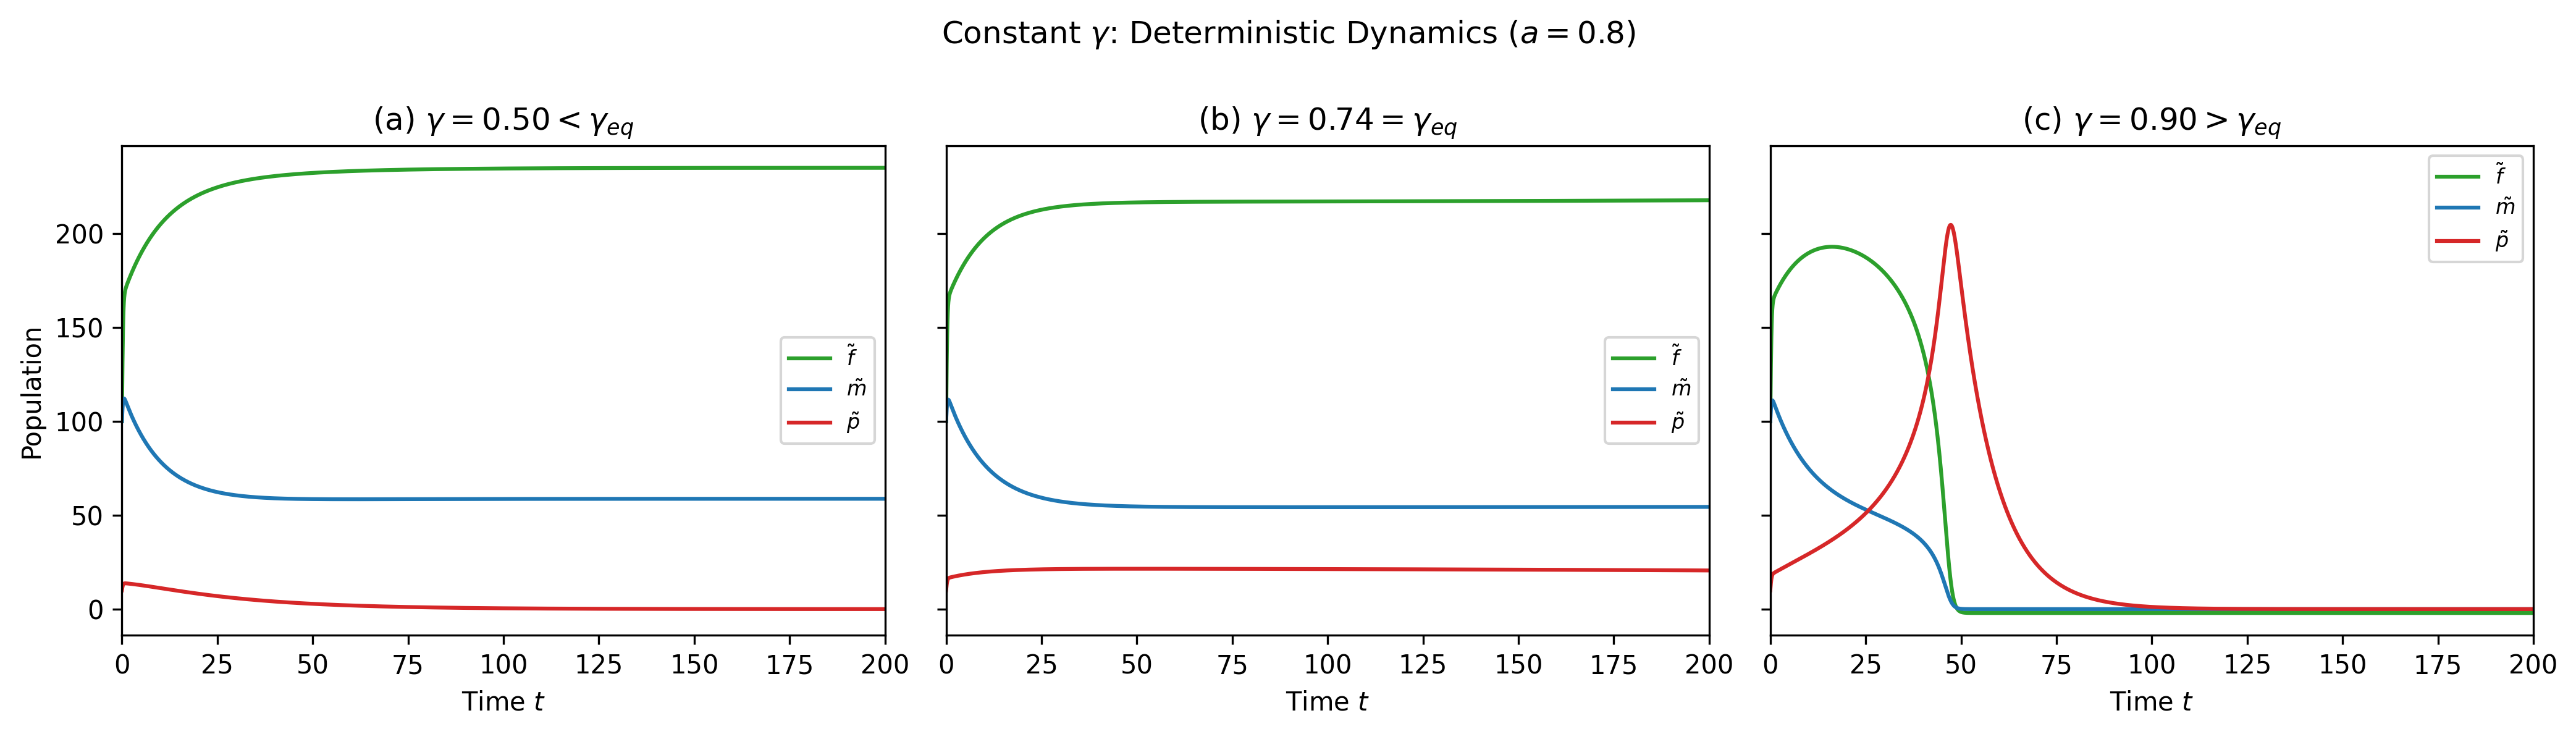
\includegraphics[width=\textwidth]{poecilia_sde/figures/fig02_constant_gamma.png}
  \caption{Constant $\gamma$ deterministic dynamics ($a = 0.8$).  (a)~$\gamma = 0.50 < \gamma_{eq}$: unisexual extinction.  (b)~$\gamma = 0.74 = \gamma_{eq}$: coexistence.  (c)~$\gamma = 0.90 > \gamma_{eq}$: bisexual then unisexual extinction.}
  \label{fig:constant_gamma}
\end{figure}

\begin{figure}[htbp]
  \centering
  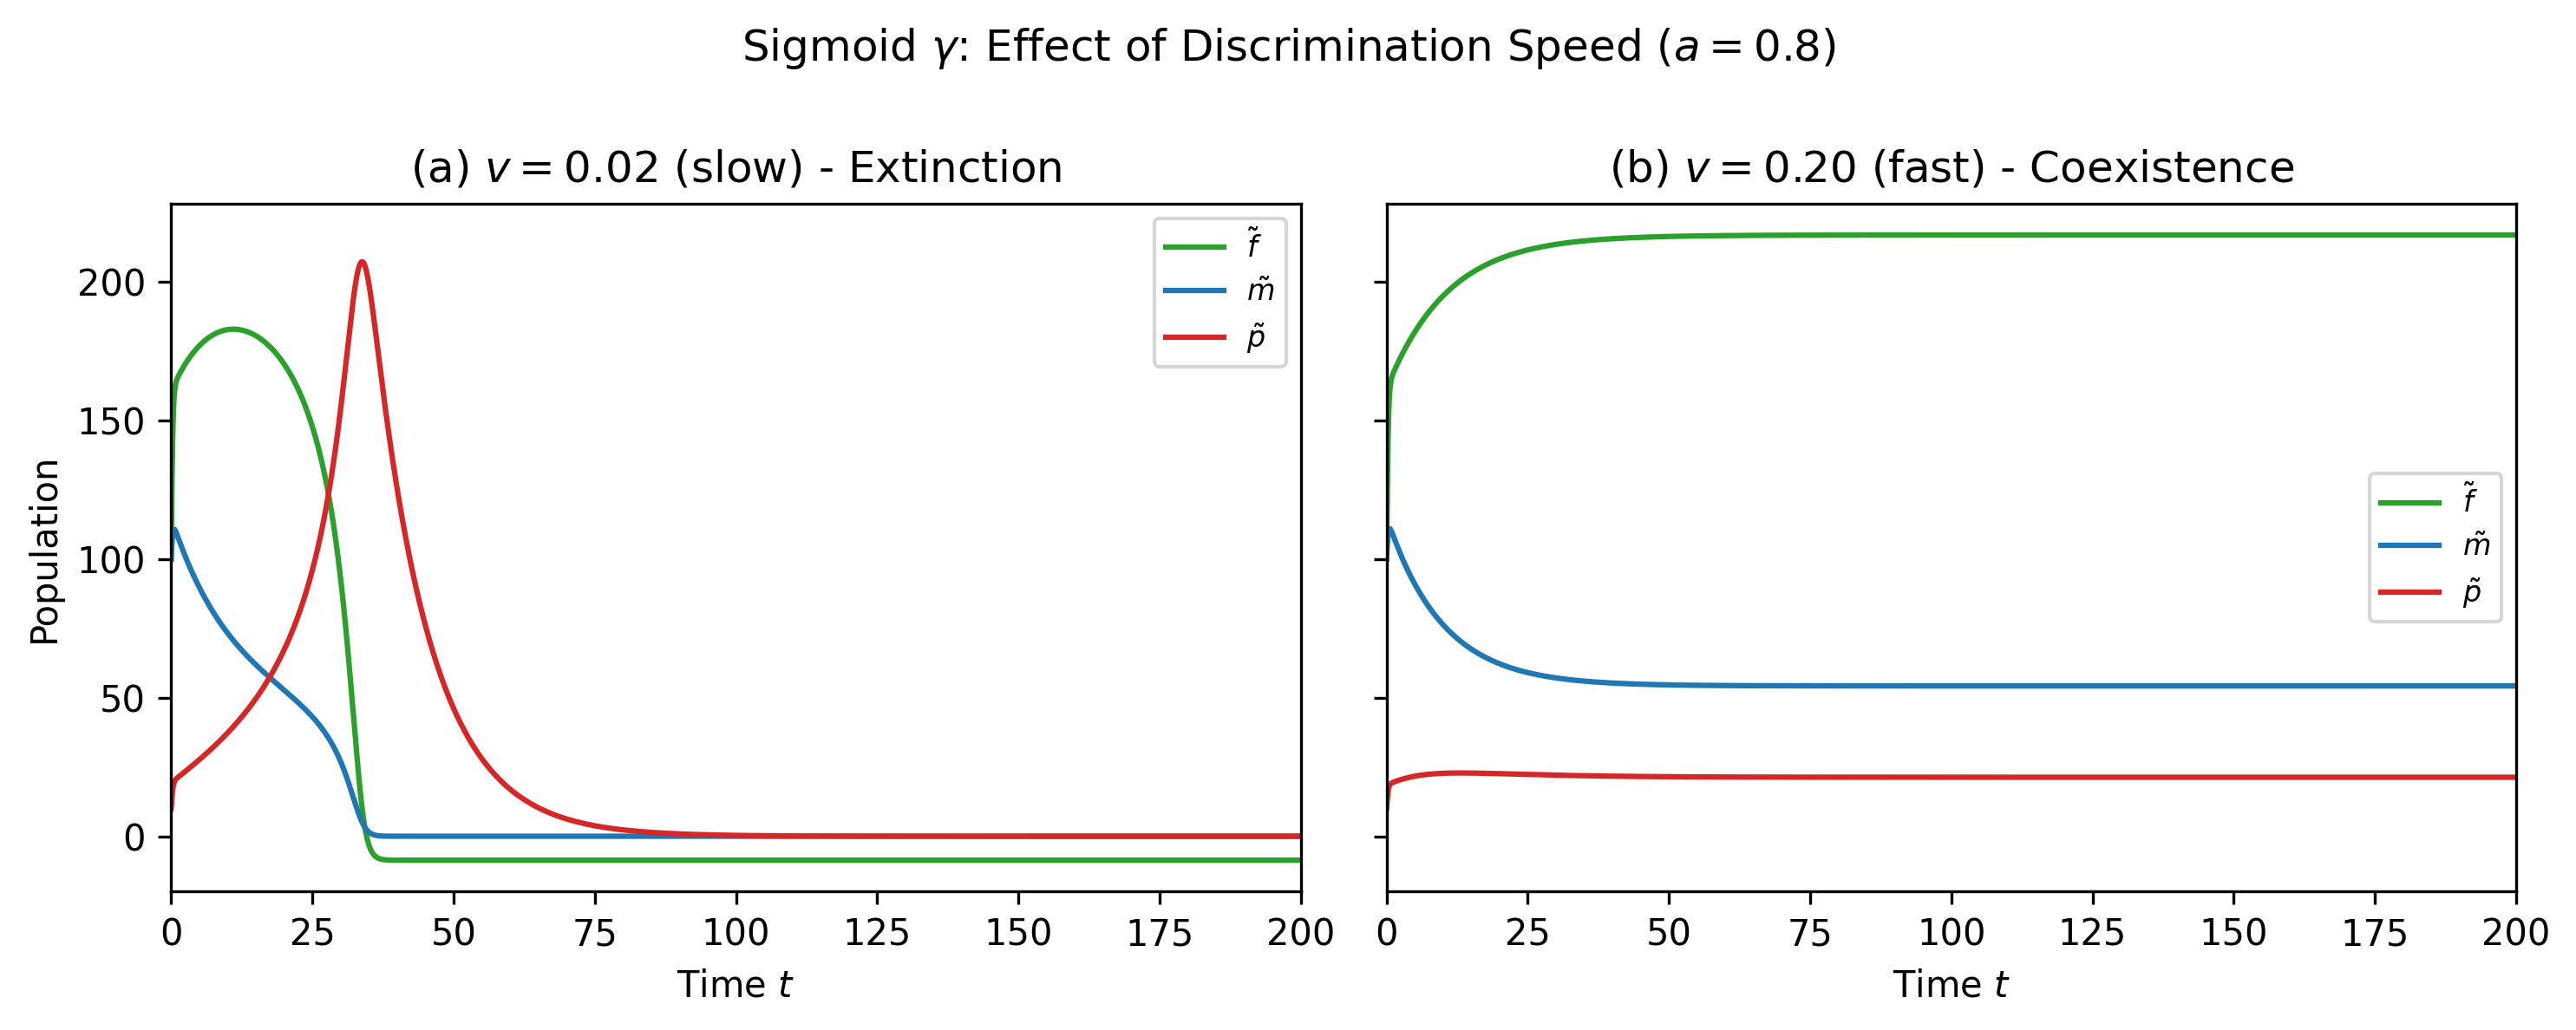
\includegraphics[width=0.85\textwidth]{poecilia_sde/figures/fig03_sigmoid_gamma.png}
  \caption{Sigmoid $\gamma$: effect of discrimination speed ($a = 0.8$).  (a)~$v = 0.02$ (slow): extinction.  (b)~$v = 0.20$ (fast): coexistence.}
  \label{fig:sigmoid_gamma}
\end{figure}

Figure~\ref{fig:rode_stochasticity} demonstrates the effect of RODE stochasticity.  With $\tilde{\eta} \in [0, 0.1]$, the non-dimensional noise sum is $\eta_f + \eta_m + \eta_p = 7/3 < 3$ (dissipative), and extinction still occurs.  With $\tilde{\eta} \in [0, 0.25]$, the sum reaches $35/6 > 3$ (threshold-exceeding), and noisy coexistence emerges---matching the high variability observed in field data.

\begin{figure}[htbp]
  \centering
  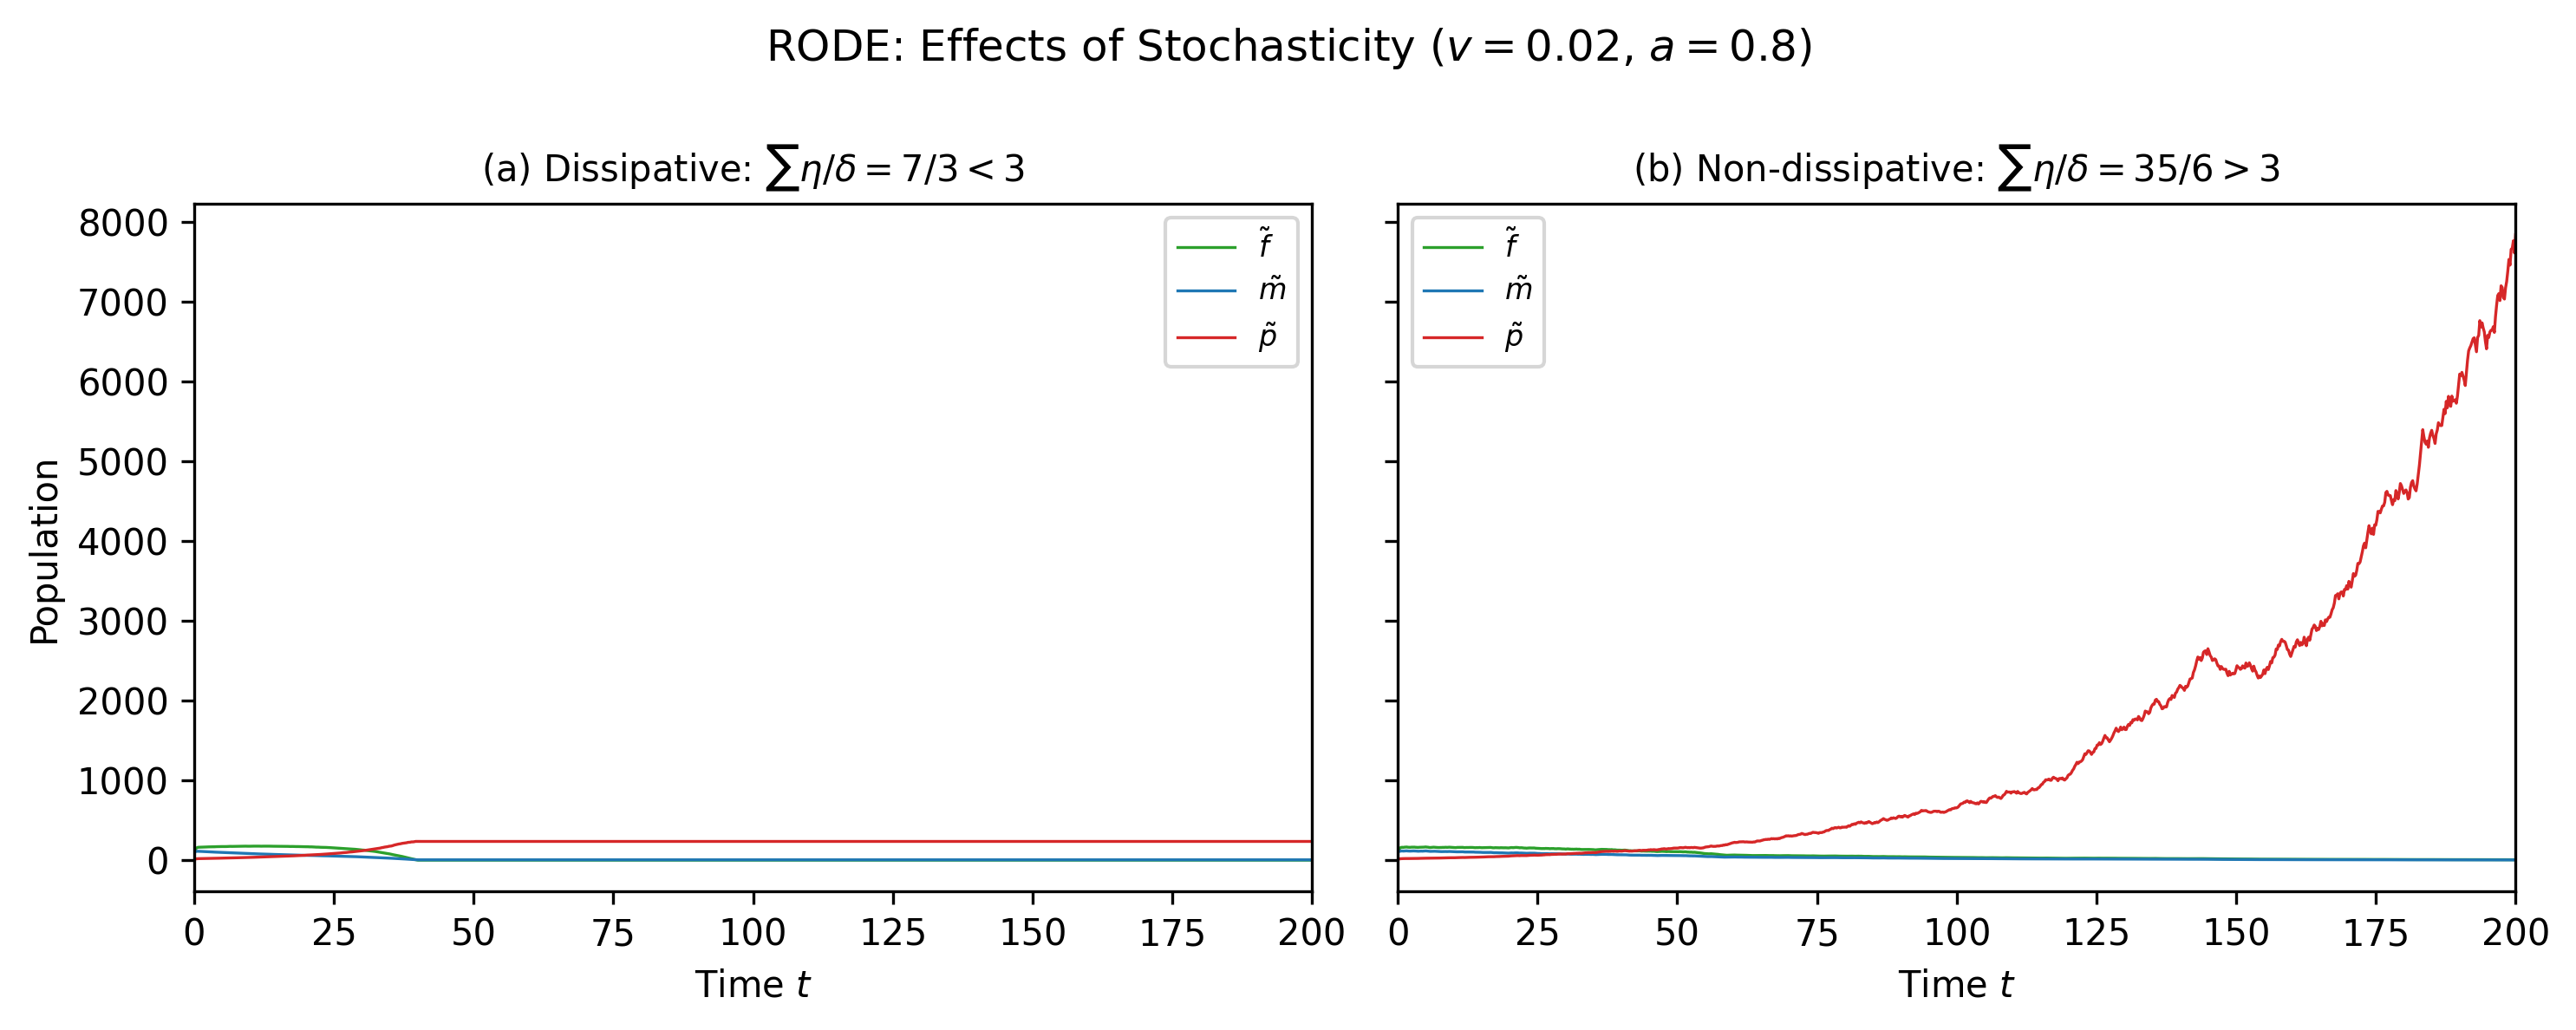
\includegraphics[width=0.85\textwidth]{poecilia_sde/figures/fig04_rode_stochasticity.png}
  \caption{RODE stochasticity ($v = 0.02$, $a = 0.8$).  (a)~Dissipative case: $\tilde{\eta}_{\max} = 0.1$, $\sum\eta/\delta = 7/3 < 3$.  (b)~Threshold-exceeding noise range: $\tilde{\eta}_{\max} = 0.25$, $\sum\eta/\delta = 35/6 > 3$.}
  \label{fig:rode_stochasticity}
\end{figure}


%---------------------------------------------------------------
\subsection{Single Trajectory Comparison}
%---------------------------------------------------------------

Figure~\ref{fig:single_trajectory} overlays single trajectories from all five formulations using the same random seed and calibrated $\sigma$ values.  While individual trajectories differ, the qualitative behavior---especially the timing and character of population transitions---is consistent across formulations.  Because the RODE noise is strictly positive-valued, RODE trajectories reflect a higher mean growth environment than the SDEs and are not expected to match SDE trajectories in absolute magnitude; the comparison targets qualitative regime membership (extinction versus coexistence) rather than quantitative agreement.  Single trajectories are inherently insufficient for quantitative comparison; they motivate the ensemble analysis that follows.

\begin{figure}[htbp]
  \centering
  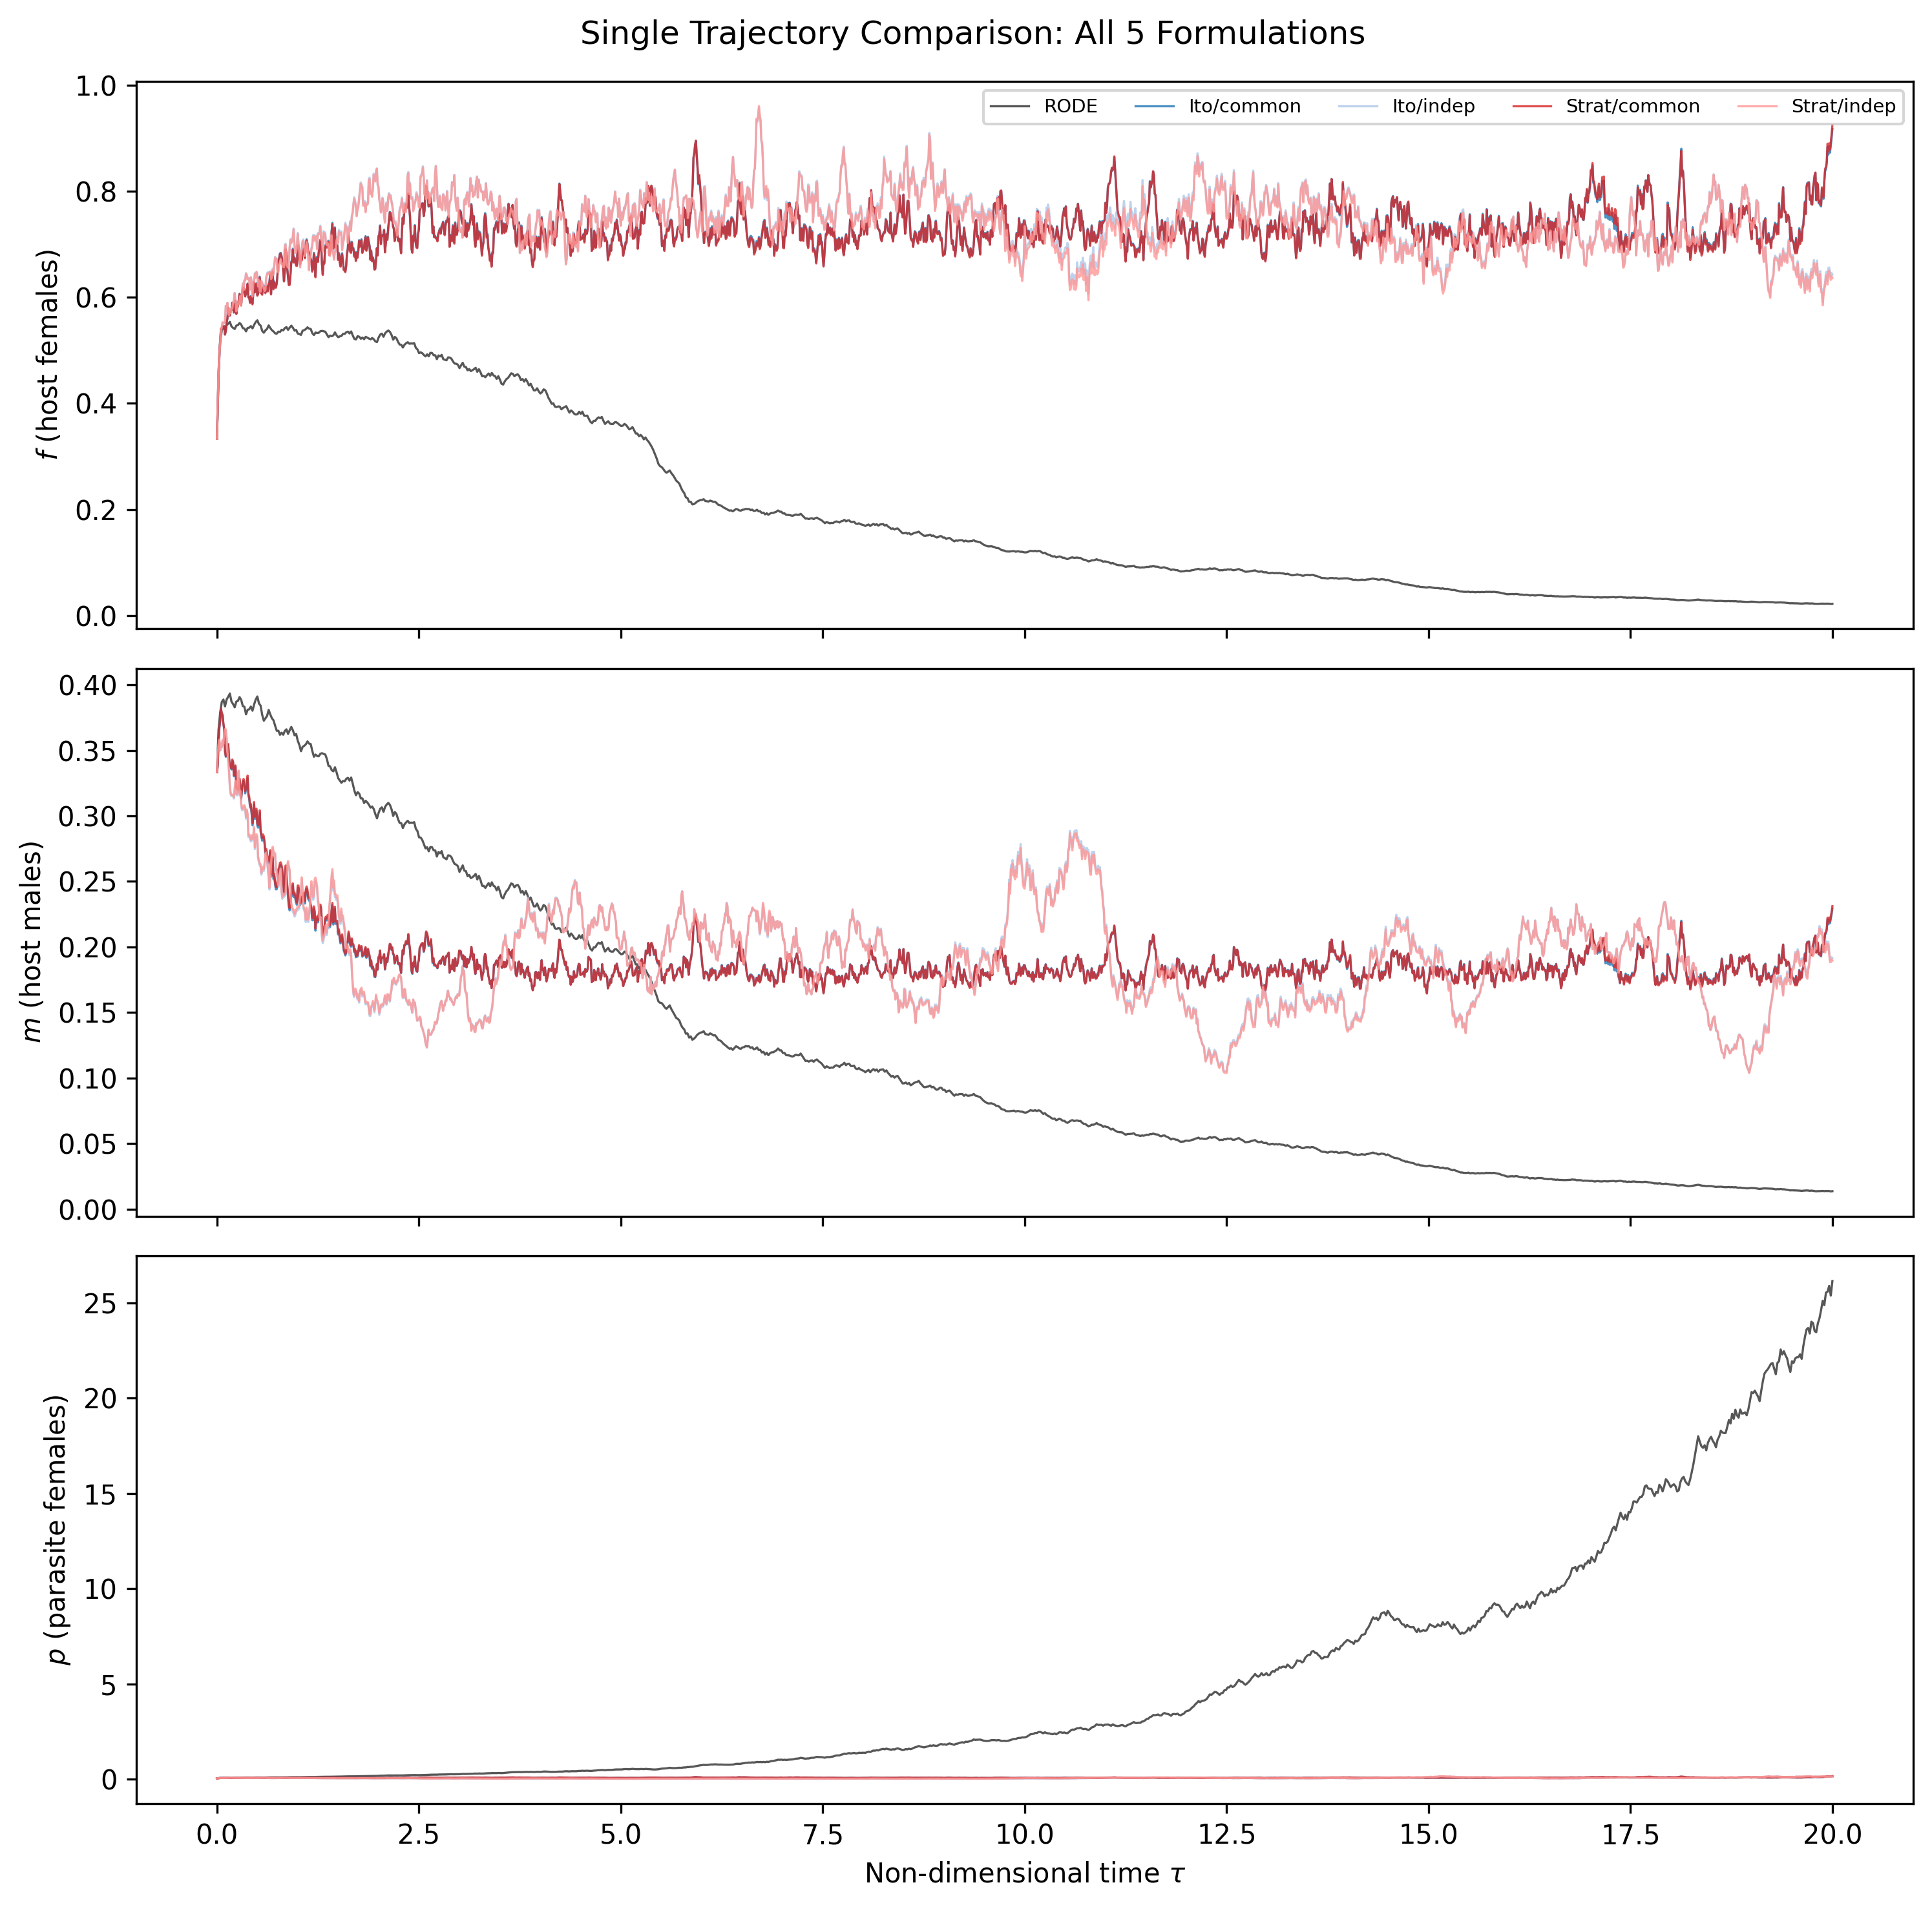
\includegraphics[width=0.85\textwidth]{poecilia_sde/figures/fig05_single_trajectory_comparison.png}
  \caption{Single trajectory comparison across all five formulations.  Rows: $f$, $m$, $p$.  Colors: RODE (dark gray), It\^{o}/common (blue), It\^{o}/independent (light blue), Stratonovich/common (red), Stratonovich/independent (light red).}
  \label{fig:single_trajectory}
\end{figure}


%---------------------------------------------------------------
\subsection{Ensemble Statistics}
%---------------------------------------------------------------

Figure~\ref{fig:ensemble_statistics} presents ensemble mean and 95\% confidence intervals for all four SDE formulations.  The It\^{o}/common and Stratonovich/common formulations show the predicted divergence in ensemble means (Propositions~\ref{prop:ito_means} and~\ref{prop:strat_means}): the Stratonovich means are systematically shifted upward by the $+\tfrac{1}{2}\sigma_i^2 F_i$ correction.  Despite this quantitative difference, all formulations agree on the extinction/coexistence classification at calibrated $\sigma$ values.

\begin{figure}[htbp]
  \centering
  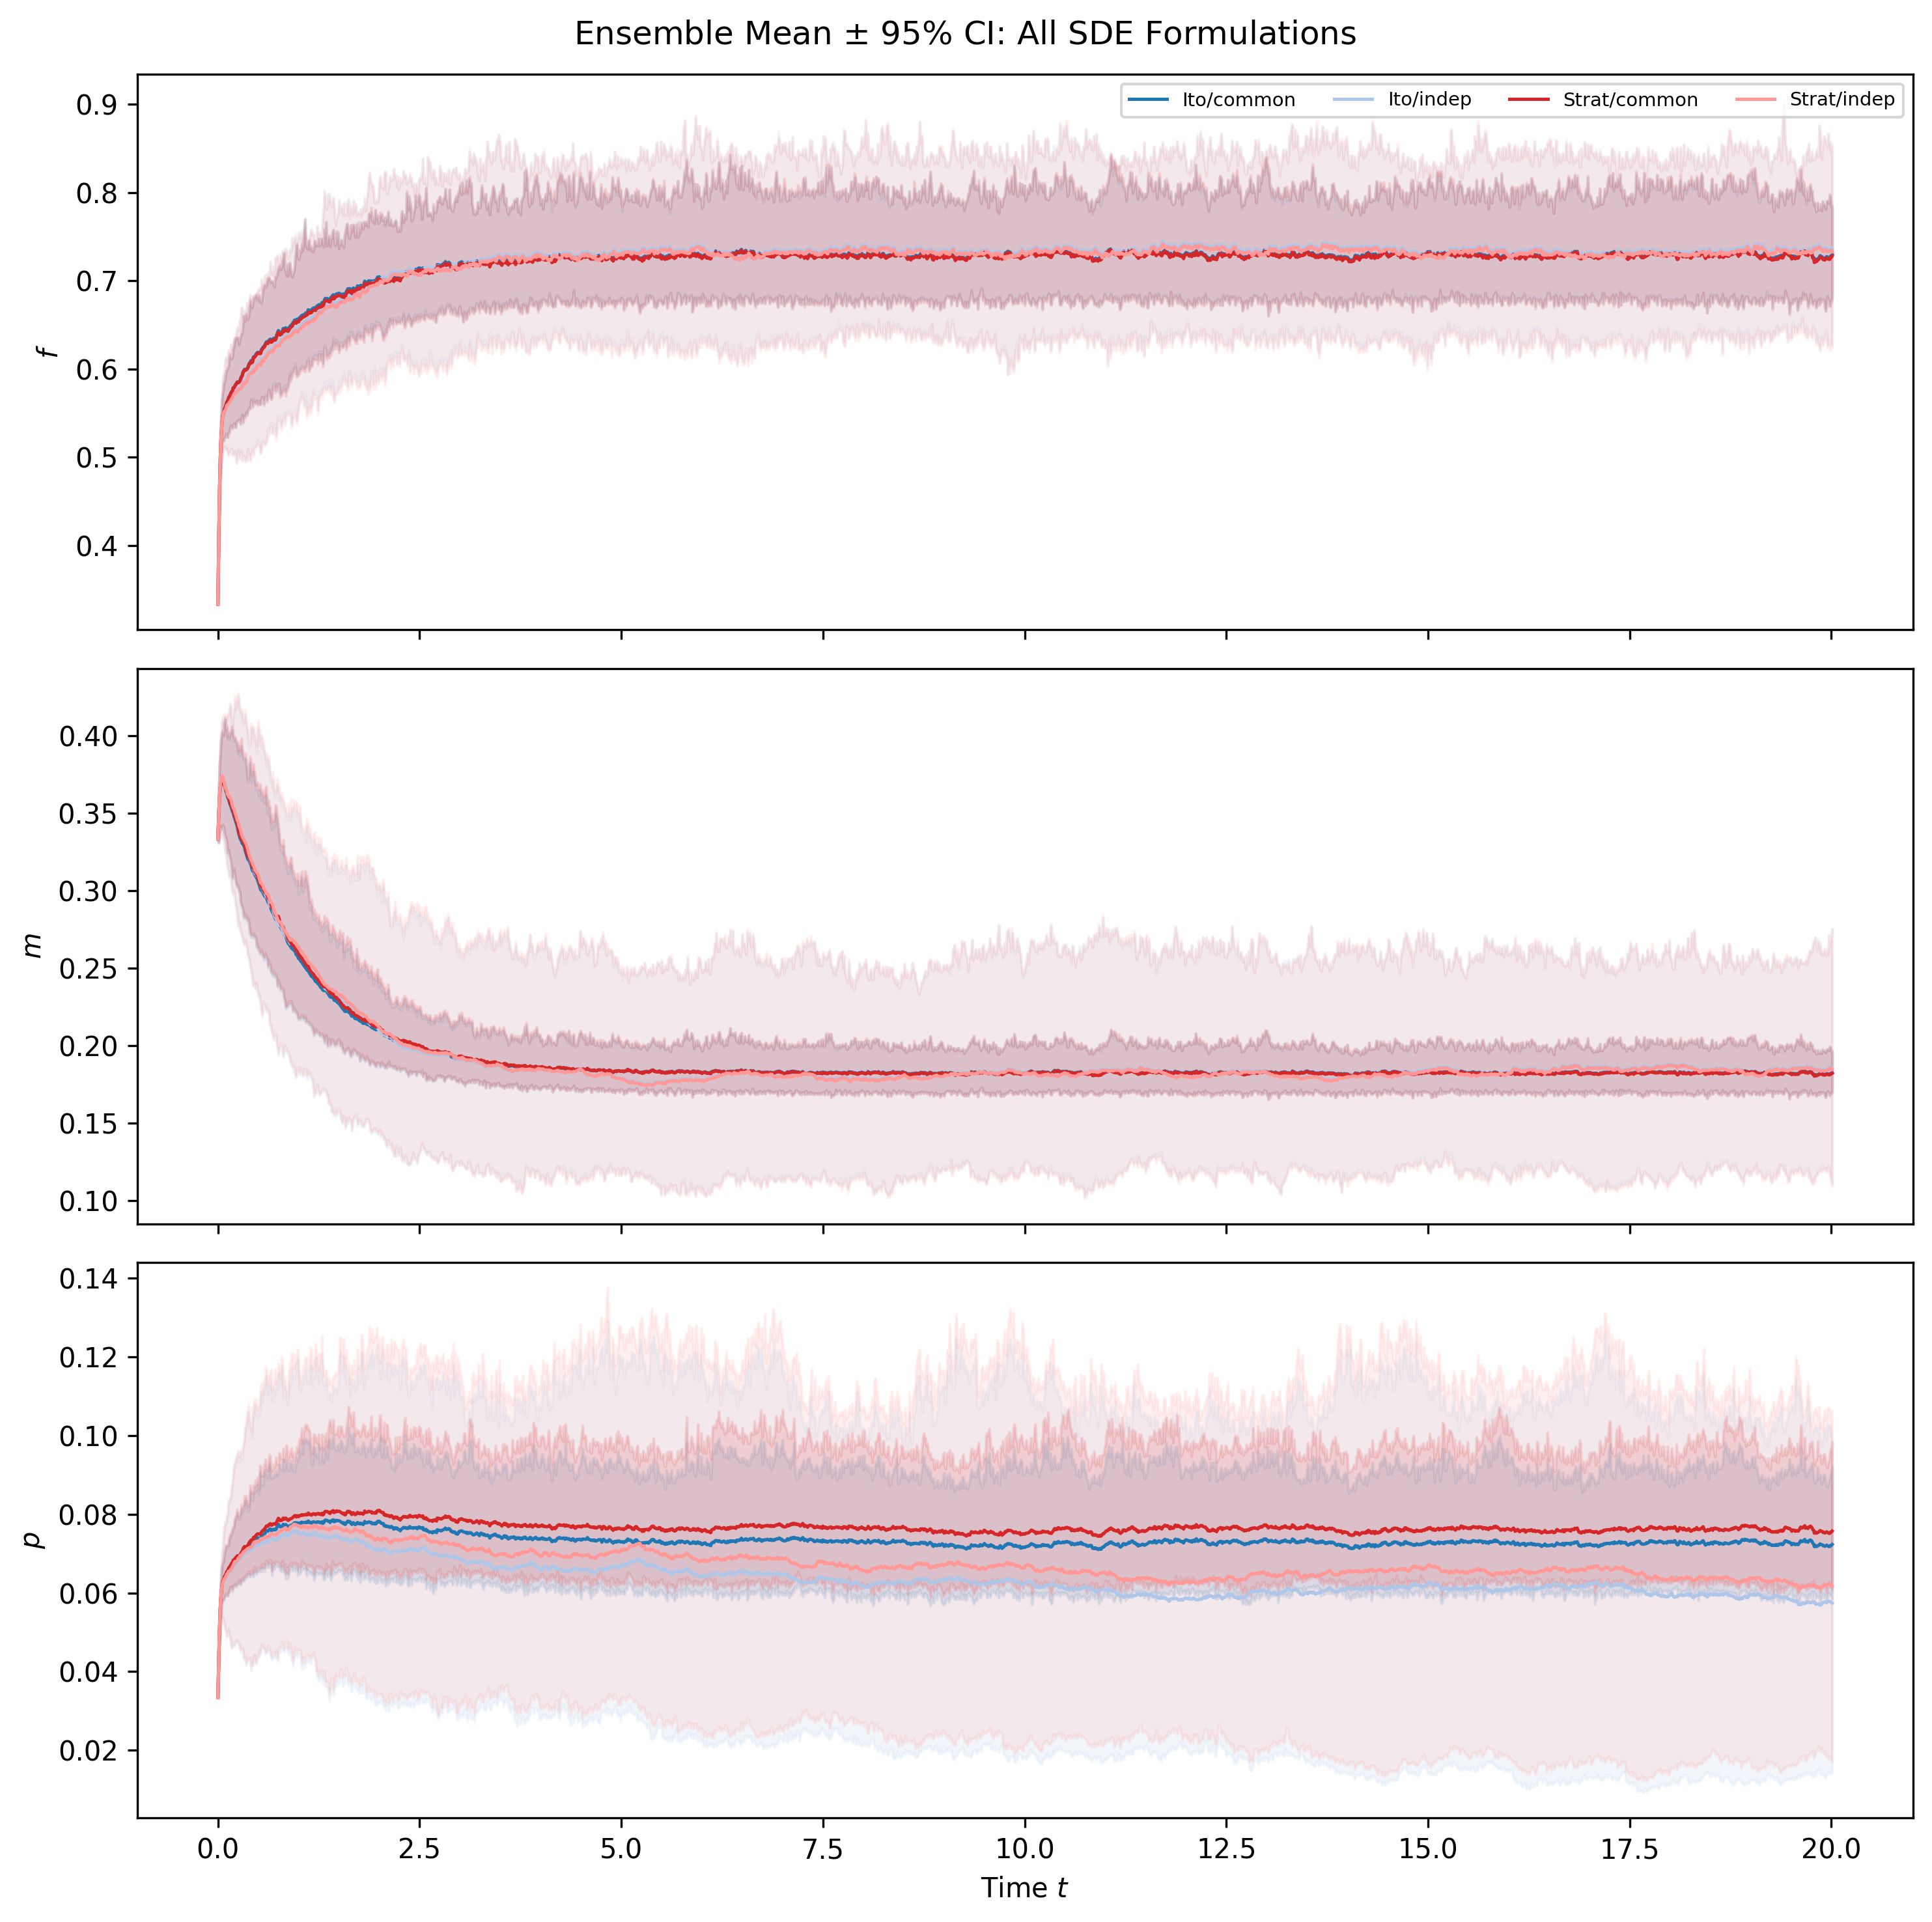
\includegraphics[width=0.85\textwidth]{poecilia_sde/figures/fig06_ensemble_statistics.png}
  \caption{Ensemble mean $\pm$ 95\% CI for all SDE formulations.  The Stratonovich means are systematically shifted upward relative to It\^{o} by the drift correction term.}
  \label{fig:ensemble_statistics}
\end{figure}


%---------------------------------------------------------------
\subsection{Moment Equations vs Monte Carlo}
%---------------------------------------------------------------

Figure~\ref{fig:moment_vs_mc} compares the diffusion-approximated moment equations against Monte Carlo ensemble statistics.  The mean equations track the Monte Carlo means well, with relative errors typically below 10\% at $t_{\text{end}}$, validating the mean-field closure for the mean dynamics.  Variance predictions diverge more, reflecting the limitations of the mean-field approximation for higher moments.

\begin{figure}[htbp]
  \centering
  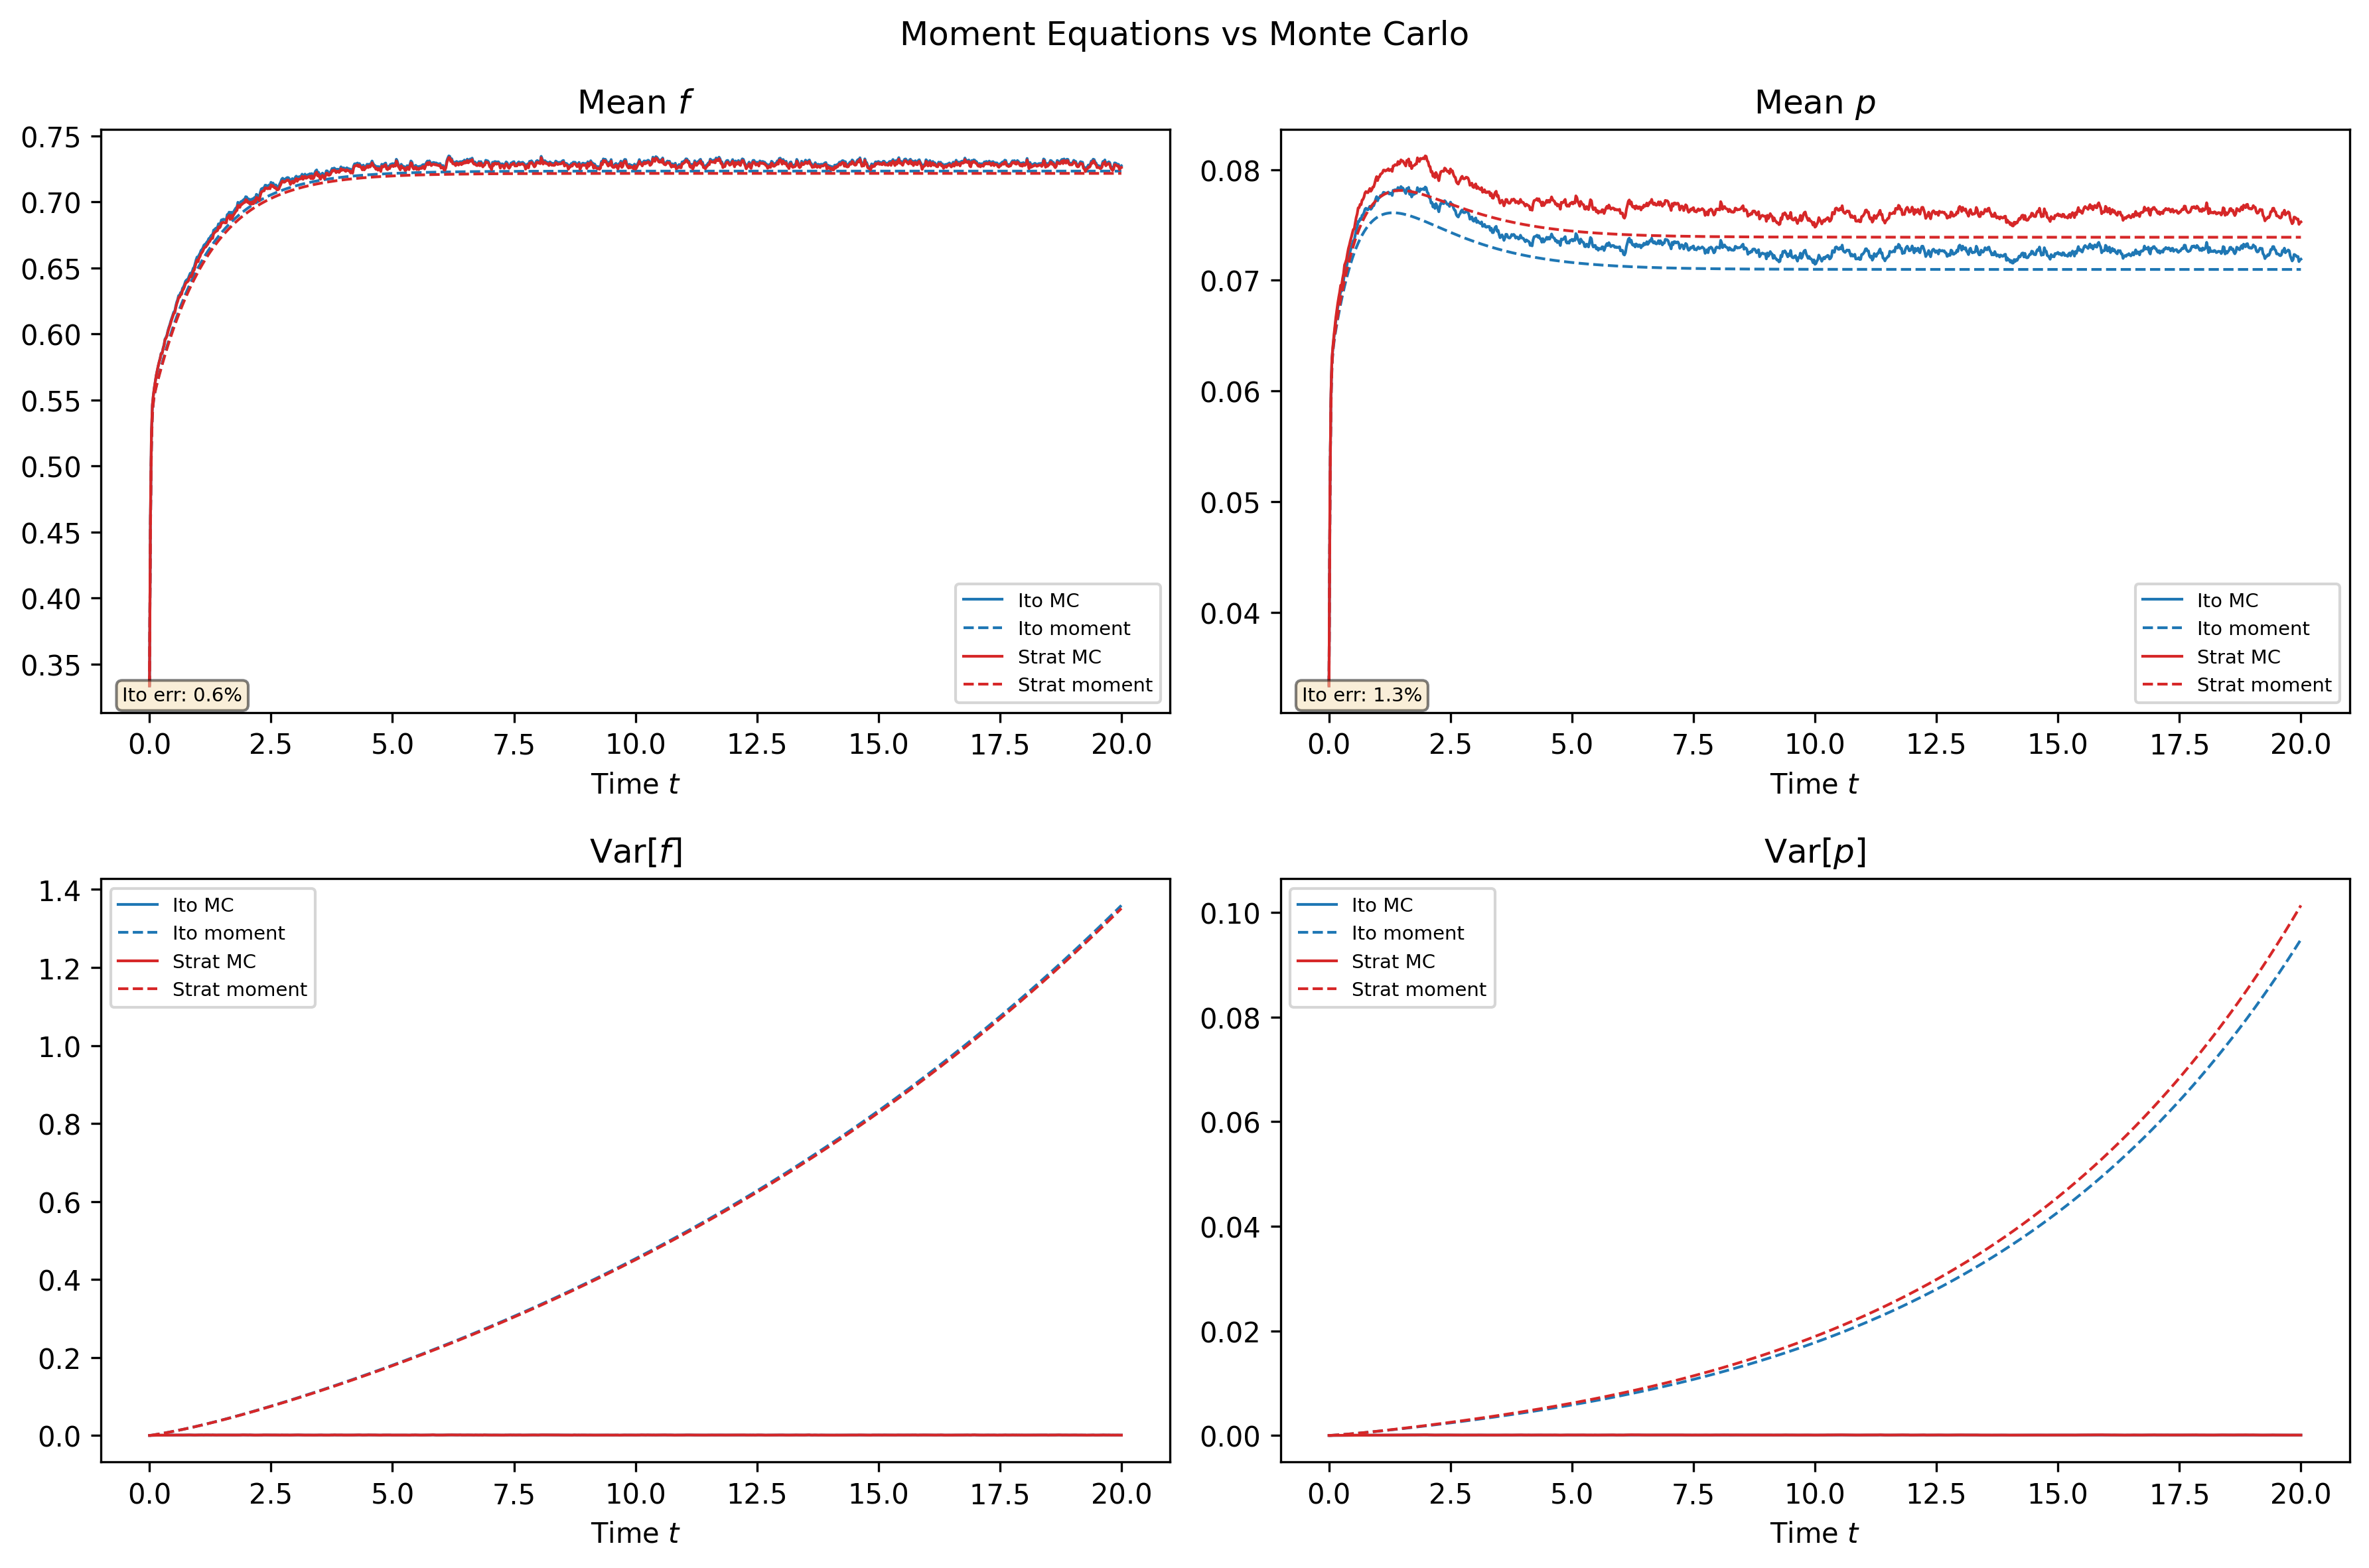
\includegraphics[width=0.85\textwidth]{poecilia_sde/figures/fig08_moment_vs_montecarlo.png}
  \caption{Moment equations (dashed) vs Monte Carlo (solid) for $f$ and $p$ populations.  Top: means.  Bottom: variances.  Text boxes show relative error at $t_{\text{end}}$.}
  \label{fig:moment_vs_mc}
\end{figure}


%---------------------------------------------------------------
\subsection{Stability Boundary}
%---------------------------------------------------------------

Figure~\ref{fig:stability_boundary} is the paper's key quantitative comparison.  It plots extinction probability as a function of noise amplitude for all four SDE formulations, with the RODE dissipative threshold shown as a vertical reference line.  The It\^{o} formulations show a clear noise-dependent stability transition: increasing $\sigma$ increases extinction probability, consistent with the $-\sigma^2/2$ shift in the Lyapunov exponent (Proposition~\ref{prop:lyap_ito}).  The Stratonovich formulations show a flatter response, consistent with the noise-independence of the Stratonovich scalar Lyapunov exponent (Proposition~\ref{prop:lyap_strat}).

\begin{figure}[htbp]
  \centering
  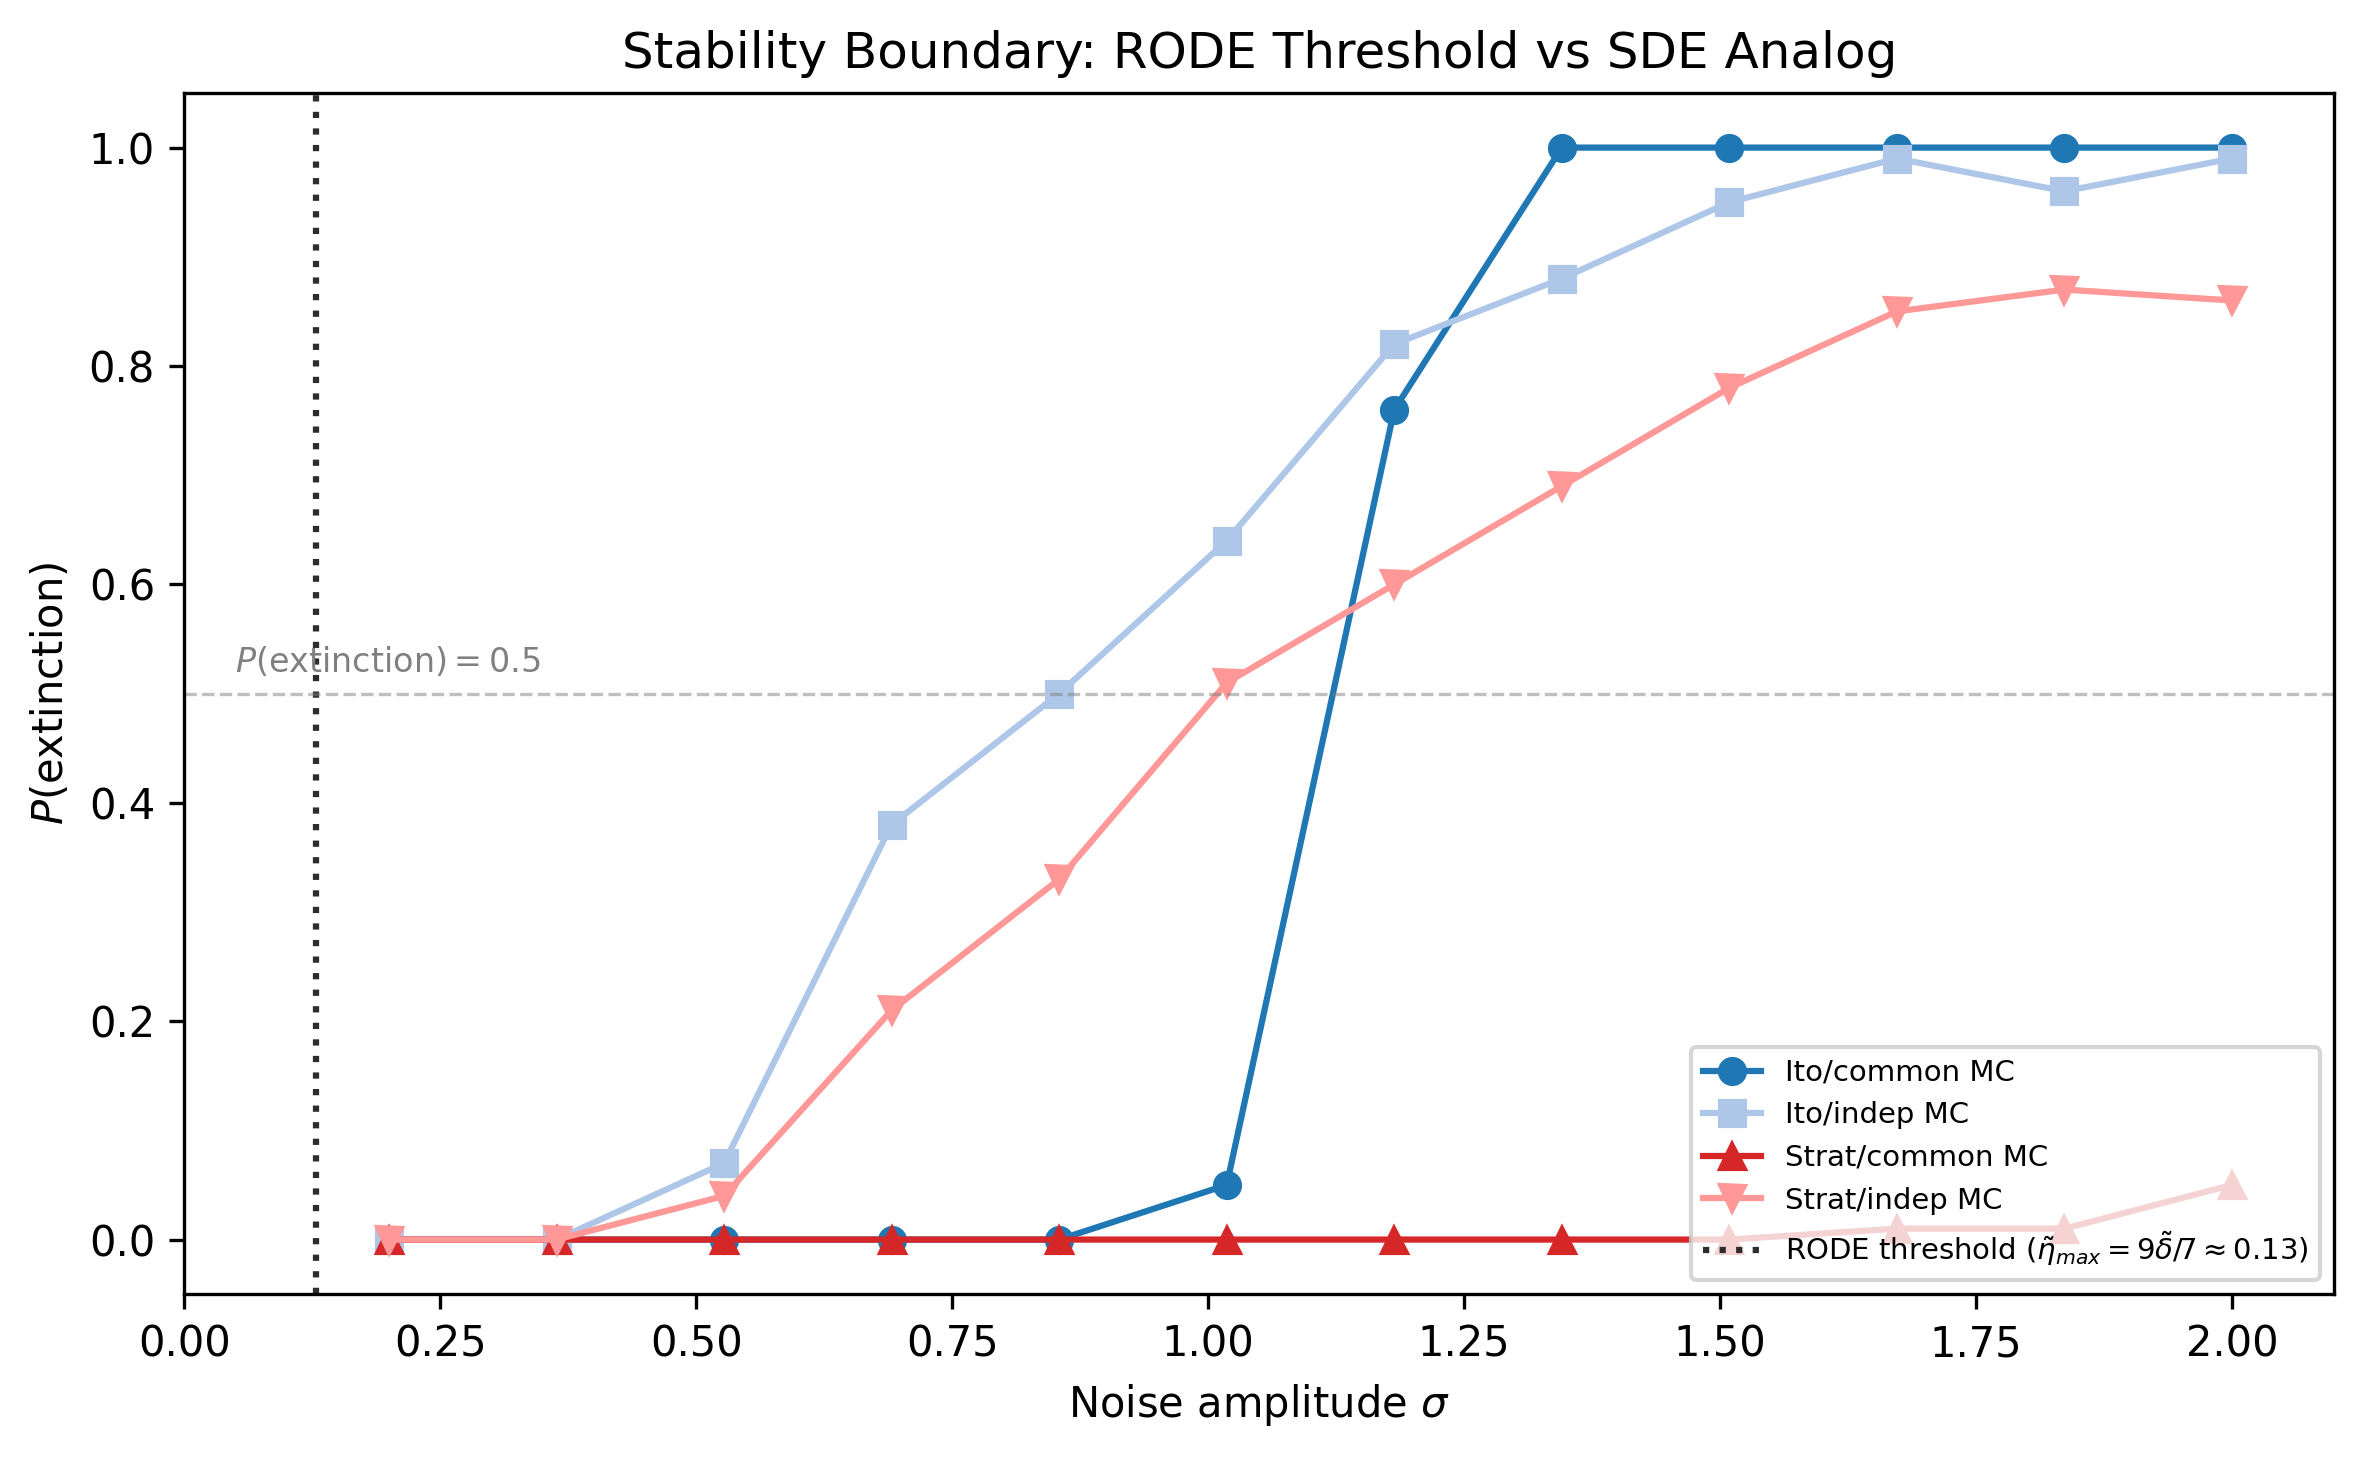
\includegraphics[width=0.7\textwidth]{poecilia_sde/figures/fig09_stability_boundary.png}
  \caption{Stability boundary comparison.  Extinction probability vs noise amplitude $\sigma$.  RODE threshold (dotted): $\tilde{\eta}_{\max} = 9\tilde{\delta}/7$.  Dashed horizontal: $P(\text{extinction}) = 0.5$.}
  \label{fig:stability_boundary}
\end{figure}


%---------------------------------------------------------------
\subsection{Noise Structure Sensitivity}
%---------------------------------------------------------------

Figure~\ref{fig:noise_sensitivity} compares common vs independent noise at exaggerated amplitude ($\sigma = 0.3$).  Common noise produces correlated fluctuations---$f$ and $p$ move together, driven by the same Wiener process---while independent noise does not.  This coherence reduces effective competition pressure in the critical regime ($p > f$), providing a mechanistic pathway for noise-stabilized coexistence not captured by the independent noise model.

\begin{figure}[htbp]
  \centering
  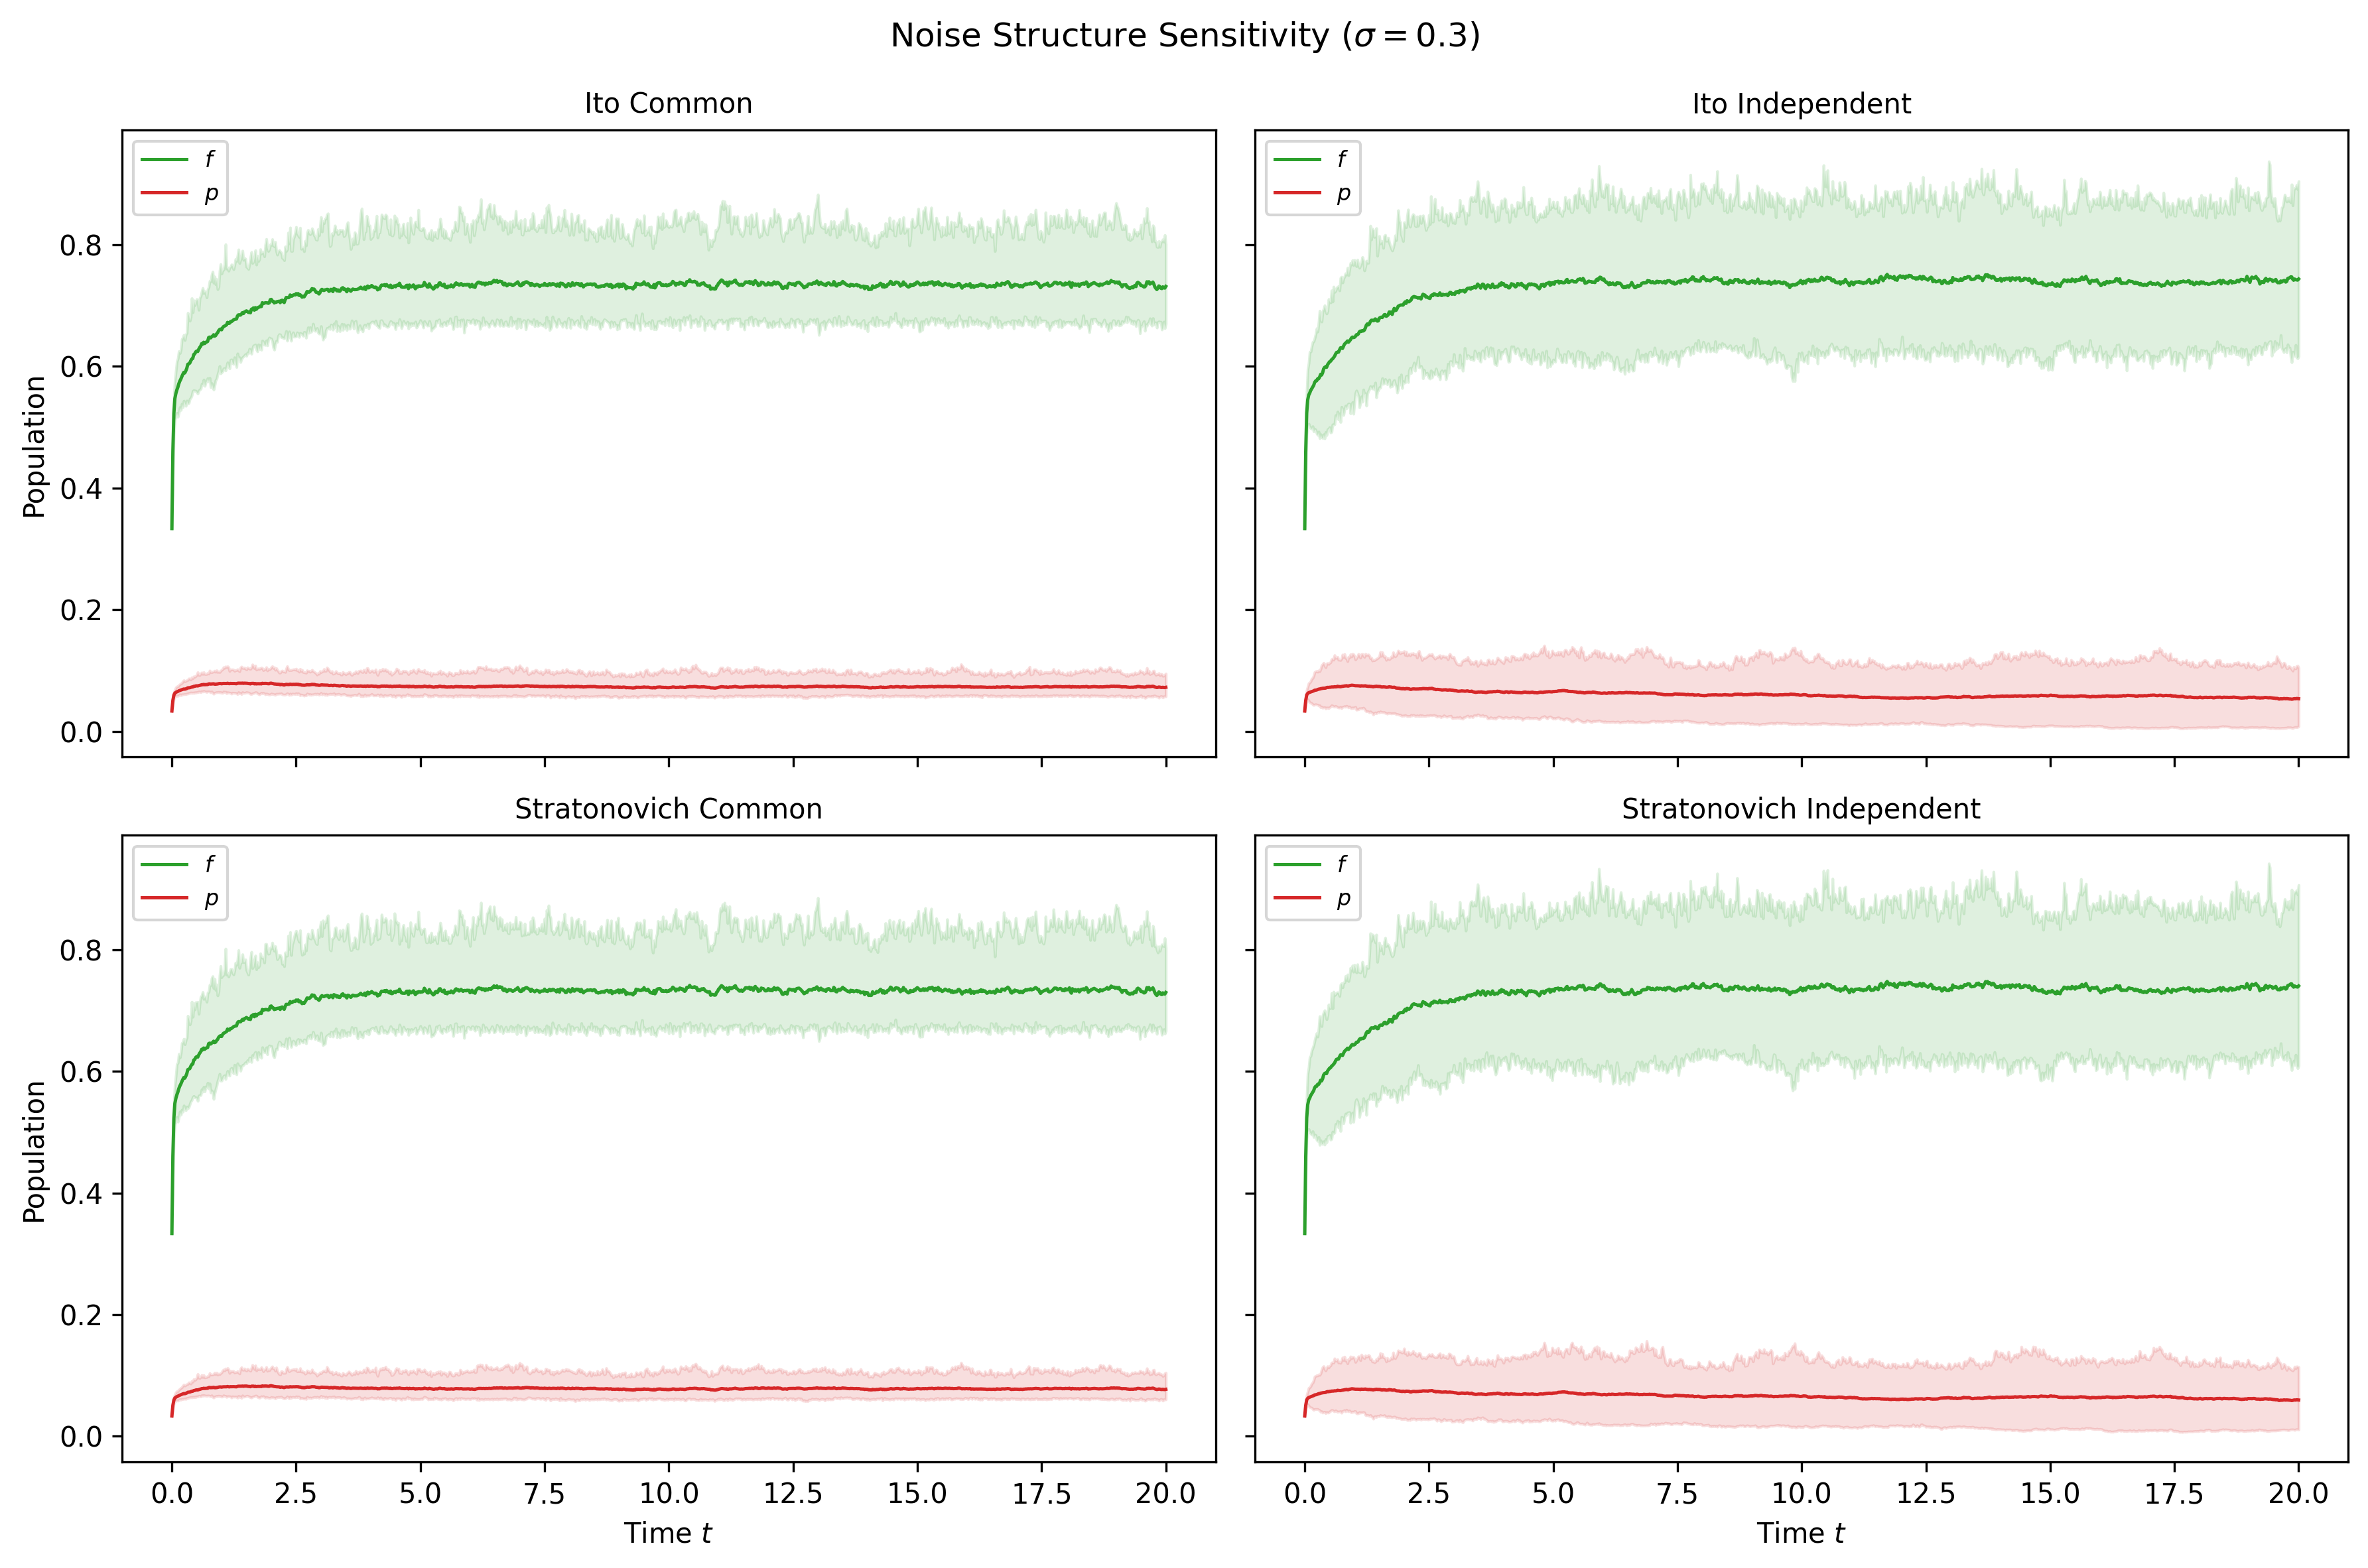
\includegraphics[width=0.85\textwidth]{poecilia_sde/figures/fig10_noise_structure_sensitivity.png}
  \caption{Noise structure sensitivity ($\sigma = 0.3$).  Common noise (left column) produces correlated $f$-$p$ fluctuations; independent noise (right) does not.}
  \label{fig:noise_sensitivity}
\end{figure}


%% =====================================================================
%% 6. DISCUSSION
%% =====================================================================
\section{Discussion}\label{sec:discussion}
%% =====================================================================
% Speed of discrimination is the master variable
The finding that the speed of male mate discrimination ($v$) governs extinction versus coexistence is robust across all five stochastic formulations tested in this study.  This parameter represents the rate at which males of the host species shift from indiscriminate mating (equal probability of mating with conspecific and parasitic females) to strong conspecific preference as the parasite population grows.  Biologically, the speed of discrimination could arise through several mechanisms: it may be a learned behavior, in which males exposed to increasing numbers of unisexual females develop discrimination through experience during their lifetime; it may be an evolved trait, in which populations with faster discrimination have been selected over evolutionary time because they are more likely to persist; or it may be a developmental response, in which environmental cues during maturation calibrate the discrimination response.  The mathematical result is unambiguous: below some critical speed the system converges to extinction regardless of initial conditions, and above this critical speed coexistence is the attractor.  This finding connects directly to field observations that some populations of \textit{P.~mexicana} coexist stably with \textit{P.~formosa} while others in nearby locations do not~\citep{Balsano1989}.  The variation in discrimination speed across field populations could be driven by several factors: local population density (higher densities may promote faster learning), prior exposure history (populations with longer coexistence histories may have evolved faster discrimination), resource availability (well-fed males may be more selective), and temperature (warmer water may accelerate learning rates).  The fact that this result is formulation-robust---it holds identically for the RODE, for both It\^{o} variants, and for both Stratonovich variants---means that the conclusion is unlikely to be an artifact of modeling choices.  Any reasonable stochastic framework applied to this system will identify discrimination speed as the master variable controlling the coexistence outcome.  This result encompasses and extends previous findings on the role of male mate discrimination~\citep{Kokko2008, Balsano1989, Kiester1981, Heubel2009}.  \citet{Heubel2009} showed that male mating efficiency matters for gynogenetic complexes; the present work sharpens this finding by demonstrating that it is the \emph{shape} of the discrimination function---specifically, the steepness of the sigmoid transition---rather than merely its asymptotic value that determines the ecological outcome.

% Noise structure and formulation-dependence
The It\^{o} and Stratonovich formulations make qualitatively different predictions about the role of noise in stabilizing or destabilizing the gynogenetic system.  In the It\^{o} framework, the Lyapunov exponent decreases by $\sigma^2/2$ with increasing noise amplitude, meaning that sufficiently intense noise can push a marginally unstable system toward extinction of the parasite---noise promotes stability of the host.  In the Stratonovich framework, the scalar Lyapunov exponent is independent of noise amplitude, and the noise-induced growth bias in the mean equations ($+\tfrac{1}{2}\sigma_i^2 F_i$) actually opposes extinction by providing an effective additional birth rate.  Which interpretation is biologically correct?  The Wong-Zakai theorem provides theoretical guidance: when the environmental signal driving population fluctuations has finite correlation time, the Stratonovich interpretation is the correct mathematical limit.  For \textit{P.~formosa} in the Soto La Marina drainage, the habitat connectivity fluctuations---pools connecting and disconnecting across the dry and wet seasons---have a correlation time on the order of weeks to months, far from the infinitesimally short correlation required for It\^{o} noise to be the natural limit.  This favors the Stratonovich interpretation, though for environmental drivers with longer correlation times an explicit random-environment (RODE-type) model may be more appropriate.  True demographic noise in birth--death count models typically scales as $\sqrt{u_i}$ in the diffusion-approximation literature; the independent multiplicative ($\sigma_i u_i$) scaling used here is appropriate for independent environmental variation in per-capita rates rather than individual birth--death events.  The implication is sobering for conservation: if Stratonovich is the correct physical model, then noise-induced stabilization of the host is not available as a mechanism, and the only stabilizing force is discrimination speed.  Environmental noise of the Stratonovich type does not shift the stability boundary, so increasing environmental variability (e.g., through climate change) would not be expected to alter the extinction/coexistence outcome.  The RODE dissipative threshold provides yet a third perspective.  The threshold $\eta_f + \eta_m + \eta_p = 3$ is based on phase-space contraction at the population ceiling---a boundary property of the vector field---rather than the linearized growth rate of a single population component near zero.  The RODE and SDE stability concepts therefore disagree fundamentally on where the boundary lies.  This disagreement is not a modeling failure: it reveals that ``stability'' is not a single concept, and different stability measures---boundary phase-space contraction, linearized growth rates, ensemble extinction probabilities---give genuinely different answers for the same biological system.  This multiplicity of stability concepts has practical implications for any ecological modeling effort that uses stochastic differential equations or random ODEs: researchers must explicitly state which stability criterion they are using and justify why that criterion is biologically relevant.

% Field data and model validation
The Balsano et al.\ (1989) field data from the Soto La Marina drainage provide the primary empirical benchmark for the model~\citep{Balsano1989}.  Across 20 locations sampled over eight years (1970--1978), the proportion of unisexuals varied from near zero to near unity, with no consistent spatial pattern and high year-to-year fluctuation even at the same site.  The ensemble variance produced by the threshold-exceeding RODE case, and by the high-$\sigma$ It\^{o} SDE case, is qualitatively consistent with this level of variability: the model produces trajectories in which the unisexual fraction swings widely, driven by the alternation between dissipative and threshold-exceeding stochastic states.  However, the model in its current form makes no prediction about which locations will be in which regime---such a prediction would require spatially resolved data on discrimination speed and habitat connectivity, which are not yet available for the Soto La Marina system.  The Travis personal communication provides an important qualitative validation (J.~Travis, personal communication): a research tank containing a stable \textit{P.~mexicana} population was accidentally contaminated with \textit{P.~formosa}, and the entire population collapsed within a year.  This observation is consistent with the model's prediction that in the absence of sufficient stochasticity (a controlled laboratory tank has minimal environmental noise), the parasitic takeover is rapid and irreversible once the parasite population exceeds the discrimination threshold.  The model has several limitations that must be acknowledged.  It does not include spatial structure; \citet{Kokko2008} demonstrated that spatial dynamics plays an important role in long-term coexistence by allowing local extinction and recolonization through a metapopulation mechanism.  The absence of spatial fragmentation is particularly relevant for the Soto La Marina system, where the seasonal cycle of pool connectivity and disconnection creates a natural spatial structure that could buffer against local extinction.  The model does not include predation, which could differentially affect the conspicuous \textit{P.~formosa} relative to the more cryptic host species, nor does it include parasite load or disease, which could further modulate population fitness in species-specific ways.  It assumes logistic growth with a single carrying capacity shared by all three populations, whereas in reality the three population types may have different resource requirements, microhabitat preferences, and competitive abilities.  Finally, the mean-field closure approximation yields acceptable accuracy for ensemble means (typically less than 10\% relative error) but underestimates variance dynamics, particularly near the extinction boundary where population distributions become highly non-Gaussian and skewed.  A Fokker-Planck analysis of the full probability density evolution would be needed to address this limitation rigorously.

% Implications for the gynogenetic eradication strategy
The analysis of the gynogenetic system provides practical insights for population management strategies based on sex-ratio manipulation.  If sperm parasites can be controlled by manipulating the discrimination speed or the noise environment, several intervention strategies become conceivable.  First, the model predicts that increasing the discrimination speed past the critical threshold should shift the system from the extinction basin to the coexistence basin.  This is a testable prediction: in aquarium experiments, populations of host males that have been pre-exposed to unisexual females (and thus have had the opportunity to develop discrimination) should show higher coexistence rates than na\"ive populations.  Second, manipulating habitat connectivity to reduce effective population size would increase the effective noise experienced by the population.  Under the It\^{o} interpretation, this would shift the stability boundary and could promote host survival; under the Stratonovich interpretation, it would have no effect on the extinction/coexistence boundary.  Mesocosm experiments comparing connected and fragmented habitat configurations could in principle distinguish between these predictions.  Third, the model shows that stochasticity alone, without sufficient discrimination speed, is insufficient for coexistence in any framework: even threshold-exceeding stochasticity cannot indefinitely prevent extinction if discrimination is too slow.  This narrows the intervention target: discrimination speed is the essential variable, and environmental manipulation is at best a complementary tool.  The sex-biased eradication strategy---in which sex-reversed individuals are introduced to drive an invasive population toward extinction by skewing the sex ratio---relies on the same dynamical mechanisms studied here.  The present results predict that target populations with slow mate discrimination are most vulnerable to such a strategy, that environments with high-amplitude (threshold-exceeding) stochasticity could stabilize coexistence and thereby undermine eradication efforts, and that the choice of stochastic framework affects quantitative predictions of the critical noise threshold but not the qualitative feasibility assessment.  These findings provide a quantitative foundation for experimental design in both conservation biology and invasive species management.


%% =====================================================================
%% 7. CONCLUSION
%% =====================================================================
\section{Conclusion}
%% =====================================================================

The speed of the sigmoid discrimination function $\gamma(p)$ is the primary determinant of extinction versus coexistence in the \textit{P.~formosa} gynogenetic system, and this conclusion is robust across all five stochastic formulations tested: the RODE with piecewise-constant noise, It\^{o} SDEs with common and independent noise, and Stratonovich SDEs with common and independent noise.  This finding reframes the coexistence problem from one about stochasticity---which is difficult to control or measure in the field---to one about behavior, which is observable and potentially subject to evolutionary selection.  The result extends the work of \citet{Heubel2009}, who showed that male mating efficiency matters for gynogenetic species complexes, by demonstrating that it is the \emph{shape} of the discrimination response (the steepness parameter $v$ of the sigmoid) rather than merely the asymptotic discrimination level $\gamma_\infty$ that governs the ecological outcome.  A testable prediction follows: populations of host males with slower discrimination response (lower $v$) should show higher extinction rates in mesocosm experiments, independent of initial population density.  This prediction could be tested by comparing host populations with different exposure histories to \textit{P.~formosa}, since prior exposure is expected to calibrate the discrimination speed.

The It\^{o} and Stratonovich stochastic calculi produce qualitatively different predictions for the role of noise in gynogenetic population stability.  It\^{o} noise induces stabilization: the scalar Lyapunov exponent decreases with noise amplitude as $\lambda_{\text{It\^{o}}} = \beta_{\text{eff}} - \delta - \tfrac{1}{2}\sigma_p^2$, meaning that sufficiently intense noise suppresses parasite growth and protects the host.  Stratonovich noise is stability-neutral for the scalar $p$-subsystem: the Lyapunov exponent $\lambda_{\text{Strat}} = \beta_{\text{eff}} - \delta$ is entirely independent of $\sigma_p$.  The choice of stochastic interpretation therefore has biological consequences, not just mathematical ones.  The Wong-Zakai theorem provides theoretical grounding for preferring the Stratonovich interpretation when environmental drivers have finite correlation time, as is the case for the seasonal habitat connectivity changes experienced by \textit{P.~formosa}~\citep{Oksendal2003}.  A testable prediction arises: mesocosm experiments with controlled environmental fluctuation timescales could in principle distinguish It\^{o}-like dynamics (high-frequency forcing, where noise amplitude affects extinction rate) from Stratonovich-like dynamics (low-frequency forcing, where noise amplitude does not affect extinction rate).  If the Stratonovich interpretation is correct, environmental noise management is irrelevant for conservation, and behavioral intervention (discrimination speed) is the only available lever.

Under mean-field closure, It\^{o} noise does not shift ensemble means relative to the deterministic system, while Stratonovich noise shifts means upward by $+\tfrac{1}{2}\sigma_i^2\,\mathbb{E}[u_i]$ per component.  This difference explains why single-trajectory simulations and ensemble averages can appear qualitatively different, and why the choice of summary statistic matters when comparing model output to field data.  The mean-field closure error is less than 10\% for the mean dynamics at the parameter values studied here, validating the closure as a useful analytical tool.  However, the closure underestimates variance dynamics, particularly near the extinction boundary where population distributions become highly skewed and non-Gaussian.  Formal analysis of closure accuracy for non-Gaussian population distributions, as arise near extinction, remains an open problem.  Future work could address this through Fokker-Planck analysis of the full probability density, or through higher-order moment closure schemes that capture skewness and kurtosis.

The RODE dissipative threshold ($\eta_f + \eta_m + \eta_p < 3$) and the It\^{o} Lyapunov threshold ($\sigma_p > \sqrt{2(\beta_{\text{eff}} - \delta)}$) are analytically distinct stability concepts that predict different boundaries even after empirical calibration.  The RODE threshold measures phase-space contraction at the population ceiling via Liouville's theorem, while the Lyapunov exponent measures linearized growth rate of the parasite population near zero.  This incommensurability is a general result: any ecological model using piecewise-constant parametric noise (RODE) should be carefully distinguished from models using Wiener-process noise (SDE), as the two frameworks have structurally different stability theories.  Our recommendation for future ecological modeling is explicit: papers that employ stochastic ODE simulation should state which stochastic framework they are using---RODE, It\^{o} SDE, or Stratonovich SDE---and justify the choice on biological grounds.  The formulation choice matters quantitatively for stability boundary predictions but not qualitatively for the ecological conclusions: across all five formulations, discrimination speed governs coexistence, and the qualitative response to noise structure (common versus independent) is the same.  This provides practical reassurance that the ecological conclusions of the present study are robust to reasonable modeling choices.


%% =====================================================================
%% APPENDICES
%% =====================================================================
\appendix

%% =====================================================================
\section{Python Implementation}\label{app:code}
%% =====================================================================
The complete implementation is organized as a flat collection of Python scripts.
All figures in this article can be reproduced by running \texttt{python run\_all.py}
after installing the packages listed in \texttt{requirements.txt}.
The scripts require Python 3.9 or later with \texttt{numpy}, \texttt{scipy},
\texttt{matplotlib}, and \texttt{sympy}.

{\footnotesize 

\subsection*{Master Script}
\lstinputlisting[language=Python,caption={run\_all.py --- master script}]
  {poecilia_sde/run_all.py}

\subsection*{Parameters}
\lstinputlisting[language=Python,caption={params.py --- parameter dataclasses}]
  {poecilia_sde/params.py}

\subsection*{Deterministic Core}
\lstinputlisting[language=Python,caption={deterministic.py --- ODE right-hand side}]
  {poecilia_sde/deterministic.py}

\subsection*{RODE Solver}
\lstinputlisting[language=Python,caption={rode.py --- Random ODE solver}]
  {poecilia_sde/rode.py}

\subsection*{It\^{o} SDE Solver}
\lstinputlisting[language=Python,caption={sde\_ito.py --- Euler--Maruyama scheme}]
  {poecilia_sde/sde_ito.py}

\subsection*{Stratonovich SDE Solver}
\lstinputlisting[language=Python,caption={sde\_stratonovich.py --- Heun scheme}]
  {poecilia_sde/sde_stratonovich.py}

\subsection*{Moment Equations}
\lstinputlisting[language=Python,caption={moments.py --- diffusion-approximated moment ODE system}]
  {poecilia_sde/moments.py}

\subsection*{Stability Analysis}
\lstinputlisting[language=Python,caption={stability.py --- stability boundary computation}]
  {poecilia_sde/stability.py}

\subsection*{Figures}
\lstinputlisting[language=Python,caption={figures.py --- all figure-generating functions}]
  {poecilia_sde/figures.py}

\subsection*{Symbolic Verification}
\lstinputlisting[language=Python,caption={verification.py --- SymPy tasks V1--V8}]
  {poecilia_sde/verification.py}

}

%% =====================================================================
\section{Numerical Methods}\label{app:numerical}
%% =====================================================================

\subsection{RODE Solver}
The RODE is solved segment by segment: noise values $\tilde{\eta}_i$ are sampled from $\mathrm{Uniform}[0, \tilde{\eta}_{\max}]$ at each evaluation point, and the ODE is integrated with \texttt{scipy.integrate.solve\_ivp} (RK45) on each interval.  Algorithm~\ref{alg:RODE} gives pseudocode.

\begin{algorithm}[H]
\DontPrintSemicolon
\SetAlgoLined
\KwIn{Parameters, $\tilde{\eta}_{\max}$, evaluation times $\{t_k\}$}
\KwOut{Solution trajectory}
$\mathbf{u} \leftarrow [\tilde{f}_0, \tilde{m}_0, \tilde{p}_0]$\;
\For{$k = 0, 1, \ldots, N-2$}{
  Sample $\tilde{\eta} \sim \mathrm{Uniform}[0, \tilde{\eta}_{\max}]$\;
  $\tilde{\eta}_f \leftarrow \tfrac{2}{3}\tilde{\eta}$, $\tilde{\eta}_m \leftarrow \tfrac{2}{3}\tilde{\eta}$, $\tilde{\eta}_p \leftarrow \tilde{\eta}$\;
  $\mathbf{u} \leftarrow \texttt{solve\_ivp}(\text{RHS}, [t_k, t_{k+1}], \mathbf{u}; \text{RK45})$\;
  $\mathbf{u} \leftarrow \max(\mathbf{u}, 0)$\;
}
\caption{RODE solver (piecewise-constant noise + RK45)}
\label{alg:RODE}
\end{algorithm}

Population values are clipped to $[0, \infty)$ after each step, and the
logistic factor is evaluated as $L = \max(1 - f - m - p,\, 0)$; the
simulated system therefore solves a truncated approximation to the smooth
analytical model.

\subsection{Step-Size Sensitivity}
All SDE results were verified by comparing ensembles with $\Delta t$ and $\Delta t/2$.  The Euler-Maruyama method has strong order 0.5~\citep{KloedenPlaten1992}, and the Heun method (Stratonovich) has strong order 1.0 for scalar multiplicative noise.  Convergence was confirmed with relative $L^2$ errors below 10\%.


%% =====================================================================
%% TABLES 2 AND 3
%% =====================================================================

\begin{table}[htbp]
  \centering
  \caption{Calibrated $\sigma$ values matching RODE threshold-exceeding variance at $T/2$.  RODE ensemble: $n = 200$ paths, $\tilde{\eta}_{\max} = 0.25$, $v = 0.02$.  SDE calibration: binary search on $\sigma$ using $n = 100$ It\^{o}/common paths.  The calibration targets the It\^{o}/common-noise variant; the same $\sigma$ tuple is then used for the remaining three SDE variants to hold noise amplitude constant across formulations.}
  \label{tab:calibration}
  \begin{tabular}{lcccc}
    \toprule
    SDE Formulation & $\sigma_f$ & $\sigma_m$ & $\sigma_p$ & Target Std$[f(T/2)]$ \\
    \midrule
    SDE variants (calibrated against It\^{o}/common; same $\sigma$ applied to other variants for cross-formulation comparison) & 0.256 & 0.256 & 0.384 & 0.031 \\
    \midrule
    \multicolumn{5}{l}{RODE reference: Std$[\tilde{f}(T/2)] = 9.30$ (dimensional), Mean$[\tilde{f}(T/2)] = 46.7$} \\
    \bottomrule
  \end{tabular}
\end{table}

\begin{table}[htbp]
  \centering
  \caption{Stability boundary summary.}
  \label{tab:stability}
  \begin{tabular}{llcc}
    \toprule
    Formulation & Noise Structure & Boundary $\sigma$ & Analytical Lyapunov \\
    \midrule
    RODE & --- & $\tilde{\eta}_{\max} = 9\tilde{\delta}/7 \approx 0.13$ & (phase-space contraction) \\
    It\^{o} & Common & $\sigma \approx 1.12$ & $\lambda = \beta_{\text{eff}} - \delta - \sigma^2/2$ \\
    It\^{o} & Independent & $\sigma \approx 0.86$ & same \\
    Stratonovich & Common & $> 2.0$ (not reached) & $\lambda = \beta_{\text{eff}} - \delta$ \\
    Stratonovich & Independent & $\sigma \approx 1.01$ & same (noise-independent) \\
    \bottomrule
  \end{tabular}
\end{table}


%% =====================================================================
%% BIBLIOGRAPHY
%% =====================================================================
\bibliographystyle{plainnat}
\bibliography{JBGInvasiveSpecies,poecilia_references}

\end{document}
